%\renewcommand{\theequation}{\theenumi}
%\begin{enumerate}[label=\arabic*.,ref=\thesection.\theenumi]
%\numberwithin{equation}{enumi}
% \renewcommand{\thefigure}{\theenumi}
% \numberwithin{figure}{enumi}
%
\item Draw Fig. \ref{fig:tri_right_angle} for $a = 4, c =3$.
\label{const:tri_right_angle}
%
\begin{figure}[!ht]
\centering
\resizebox{\columnwidth}{!}{%Code by GVV Sharma
%December 6, 2019
%released under GNU GPL
%Drawing a right angled triangle

\begin{tikzpicture}[scale=2]

%Triangle sides
\def\a{4}
\def\c{3}

%Marking coordiantes
\coordinate [label=above:$A$] (A) at (0,\c);
\coordinate [label=left:$B$] (B) at (0,0);
\coordinate [label=right:$C$] (C) at (\a,0);

%Drawing triangle ABC
\draw (A) -- node[left] {$\textrm{c}$} (B) -- node[below] {$\textrm{a}$} (C) -- node[above,,xshift=2mm] {$\textrm{b}$} (A);

%Drawing and marking angles
\tkzMarkAngle[fill=orange!40,size=0.5cm,mark=](A,C,B)
\tkzMarkRightAngle[fill=blue!20,size=.3](A,B,C)
\tkzLabelAngle[pos=0.65](A,C,B){$\theta$}
\end{tikzpicture}
}
\caption{Right Angled Triangle}
\label{fig:tri_right_angle}	
\end{figure}
\\
\solution The vertices of $\triangle ABC$ are 
\begin{align}
\vec{A} = \myvec{0\\c} = \myvec{0\\3}, \vec{B} = \myvec{0\\0}, \vec{C} = \myvec{a\\0}=\myvec{4\\0}
\end{align}
%
The python code for  Fig. \ref{fig:tri_right_angle} is
\begin{lstlisting}
codes/triangle/tri_right_angle.py
\end{lstlisting}
%
and the equivalent latex-tikz code is
%
\begin{lstlisting}
figs/triangle/tri_right_angle.tex
\end{lstlisting}
%
The above latex code can be compiled as a standalone document as
%
\begin{lstlisting}
figs/triangle/tri_right_angle_alone.tex
\end{lstlisting}
%

\item Draw Fig. \ref{fig:tri_polar} for $a = 4, c =3$.
\label{const:tri_polar}
%
\\
\solution 
 The vertex  $\vec{A}$ can  be expressed  in {\em polar coordinate form} as
%\label{prob:tri_polar}
%
\begin{align}
\vec{A} = b\myvec{\cos \theta\\  \sin \theta} 
\end{align}
%
where
\begin{align}
b = \sqrt{a^2+c^2} = 5, \tan \theta = \frac{3}{4}
\end{align}
%The vertices of $\triangle ABC$ are 
%\begin{align}
%\vec{A} = \myvec{a\\c} = \myvec{4\\3}, \vec{B} = \myvec{a\\0}  = \myvec{4\\0}, \vec{C} = \myvec{0\\0}.
%\end{align}
%
The python code for  Fig. \ref{fig:tri_polar} is
\begin{lstlisting}
codes/triangle/tri_polar.py
\end{lstlisting}
%
and the equivalent latex-tikz code is
%
\begin{lstlisting}
figs/triangle/tri_polar.tex
\end{lstlisting}
\begin{figure}[!ht]
\centering
\resizebox{\columnwidth}{!}{%Code by GVV Sharma
%December 6, 2019
%released under GNU GPL
%Drawing a right angled triangle

\begin{tikzpicture}[scale=2]

%Triangle sides
\def\a{4}
\def\c{3}

%Marking coordiantes
\coordinate [label=above:$A$] (A) at (\a,\c);
\coordinate [label=below:$B$] (B) at (\a,0);
\coordinate [label=left:$C$] (C) at (0,0);

%Drawing triangle ABC
\draw (A) -- node[left] {$\textrm{c}$} (B) -- node[below] {$\textrm{a}$} (C) -- node[above left,xshift=2mm] {$\textrm{b}$} (A);

%Drawing and marking angles
\tkzMarkAngle[fill=orange!40,size=0.5cm,mark=](B,C,A)
\tkzMarkRightAngle[fill=blue!20,size=.3](A,B,C)
\tkzLabelAngle[pos=0.65](A,C,B){$\theta$}
\end{tikzpicture}
}
\caption{Right Angled Triangle}
\label{fig:tri_polar}	
\end{figure}
%
\item Draw Fig. \ref{fig:tri_sss} with $a=6$, $b=5$  and $c=4$.  
\label{const:tri_sss}
\begin{figure}[!ht]
	\begin{center}
			\resizebox{\columnwidth}{!}{%Code by GVV Sharma
%December 7, 2019
%released under GNU GPL
%Drawing a triangle given 3 sides

\begin{tikzpicture}
[scale=2,>=stealth,point/.style={draw,circle,fill = black,inner sep=0.5pt},]

%Triangle sides
\def\a{6}
\def\b{5}
\def\c{4}
 
%Coordinates of A
%\def\p{{\a^2+\c^2-\b^2}/{(2*\a)}}
\def\p{2.25}
\def\q{{sqrt(\c^2-\p^2)}}

%Labeling points
\node (A) at (\p,\q)[point,label=above right:$A$] {};
\node (B) at (0, 0)[point,label=below left:$B$] {};
\node (C) at (\a, 0)[point,label=below right:$C$] {};

%Foot of perpendicular

\node (D) at (\p,0)[point,label=above right:$D$] {};

%Drawing triangle ABC
\draw (A) -- node[left] {$\textrm{c}$} (B) -- node[below] {$\textrm{a}$} (C) -- node[above,xshift=2mm] {$\textrm{b}$} (A);

%Drawing altitude AD
\draw (A) -- node[left] {$\textrm{h}$}(D);

%Drawing and marking angles
%\tkzMarkAngle[fill=orange!40,size=0.5cm,mark=](A,C,B)
%\tkzMarkAngle[fill=orange!40,size=0.4cm,mark=](D,B,A)
%\tkzMarkAngle[fill=green!40,size=0.5cm,mark=](B,A,C)
%\tkzMarkAngle[fill=green!40,size=0.5cm,mark=](C,B,D)
\tkzMarkRightAngle[fill=blue!20,size=.2](A,D,B)
%\tkzMarkRightAngle[fill=blue!20,size=.2](B,D,A)
%\tkzLabelAngle[pos=0.65](A,C,B){$\theta$}
%\tkzLabelAngle[pos=0.65](A,B,D){$\theta$}
%\tkzLabelAngle[pos=1](B,A,C){\rotatebox{-45}{$\alpha = 90\degree -\theta$}}
%\tkzLabelAngle[pos=0.65](C,B,D){$\alpha$}

\end{tikzpicture}
}
	\end{center}
	\caption{}
	\label{fig:tri_sss}	
\end{figure}
\\
\solution Let the vertices of  $\triangle ABC$ and $\vec{D}$ be 
\begin{align}
\label{eq:tri_basic}
\vec{A} = \myvec{p\\q}, \vec{B} = \myvec{0\\0}, \vec{C} = \myvec{a\\0}, \vec{D} = \myvec{p\\0}
\end{align}
%

Then
\begin{align}
\label{eq:c_tricoord}
AB &= \norm{\vec{A}-\vec{B}}^2 = \norm{\vec{A}}^2  = c^2 \quad \because \vec{B} = \vec{0}
\\
\label{eq:a_tricoord}
BC &= \norm{\vec{C}-\vec{B}}^2 = \norm{\vec{C}}^2  = a^2
\\
AC &= \norm{\vec{A}-\vec{C}}^2 =    b^2
\label{eq:b_tricoord}
\end{align}
%
From \eqref{eq:b_tricoord},
\begin{align}
b^2 &=\norm{\vec{A}-\vec{C}}^2 = \norm{\vec{A}-\vec{C}}^T\norm{\vec{A}-\vec{C}}  
\\
&= \vec{A}^T\vec{A}+\vec{C}^T\vec{C}-\vec{A}^T\vec{C} - \vec{C}^T\vec{A} 
\\
&= \norm{\vec{A}}^2 + \norm{\vec{C}}^2 - 2\vec{A}^T\vec{C} \quad \brak{\because \vec{A}^T\vec{C} = \vec{C}^T\vec{A} } 
\label{eq:tri_const_norm_ac}
\\
&= a^2+c^2-2ap
\end{align}
%
yielding
\begin{align}
p&= \frac{a^2+c^2-b^2}{2a}
\end{align}
%
From \eqref{eq:c_tricoord}, 
\begin{align}
\norm{\vec{A}}^2 &= c^2 = p^2+q^2
\\
\implies q&= \pm \sqrt{c^2-p^2}
\end{align}
%
The python code for  Fig. \ref{fig:tri_sss} is
\begin{lstlisting}
codes/triangle/tri_sss.py
\end{lstlisting}
%
and the equivalent latex-tikz code is
%
\begin{lstlisting}
figs/triangle/tri_sss.tex
\end{lstlisting}

\item Construct a triangle of sides $a=4$, $b=5$  and $c=6$.  
\\
\solution

\begin{table}[!ht]
\centering
\resizebox{\columnwidth}{!}{\begin{tabular}{|c|c|c|c|} 
\hline
kind of  cake & No.of cakes & Flour& Fat\\
\hline
1st & x & 200g  &  25g \\ 
\hline
2nd& y& 100g&  50g  \\ 
\hline
Total& x+y& 5 kg=5000g&1kg=1000g \\ 
\hline
\end{tabular}}
\caption{Ingredients used in making the cake is flour and fat }
\label{opt/13/tab:table1}
\end{table}
Let the  1st kind  be $x$ and the 2nd kind be $y$  such that 
\begin{align}
x \geq 0 \\
y \geq 0 
\end{align}
According to the question,
\begin{align}
2{x} + {y} \leq 50
\\
{x} + 2{y} \leq 40
\end{align}
$\therefore$ Our problem is
\begin{align}
\max_{\vec{x}} Z &= \myvec{1& 1}\vec{x}\\
s.t. \quad \myvec{2 & 1 \\ 1& 2}\vec{x} &\preceq \myvec{50\\40} 
\end{align}
Lagrangian function is given by
\begin{equation}
\begin{aligned}
&L(\vec{x},\boldsymbol{\lambda}) \\ &= \myvec{1 & 1}\vec{x}+\lcbrak{\sbrak{\myvec{2 & 1}\vec{x}-50}} \\ &+ \sbrak{\myvec{1 & 2}\vec{x}-40}\\ &+ \sbrak{\myvec{-1 & 0}\vec{x}} +\rcbrak{\sbrak{\myvec{0 & -1}\vec{x}}}\boldsymbol{\lambda}
\end{aligned}
\end{equation}
where,
\begin{align}
\boldsymbol{\lambda} &= \myvec{\lambda_1 \\ \lambda_2 \\ \lambda_3 \\ \lambda_4 \\ \lambda_5 \\ \lambda_6}
\end{align}
Now,
\begin{align}
\nabla L(\vec{x},\boldsymbol{\lambda}) &= \myvec{1+ \myvec{2 & 1 & -1 & 0 }\boldsymbol{\lambda}\\ 1+\myvec{1 & 2 & 0 & -1}\boldsymbol{\lambda} \\ \myvec{2 & 1}\vec{x}-50\\ \myvec{1& 2}\vec{x}-40 \\  \myvec{-1 & 0}\vec{x} \\ \myvec{0 & -1}\vec{x}}
\end{align}
$\therefore$ Lagrangian matrix is given by
\begin{align}
\myvec{0 & 0 & 2 & 1& -1 & 0 \\ 0 & 0 & 1 & 2  & 0 & -1 \\ 2 & 1 & 0 & 0 & 0 & 0 \\ 1 & 2 & 0 & 0 & 0 & 0  \\ -1 & 0 & 0 & 0 & 0 & 0  \\ 0 & -1 & 0 & 0 & 0 & 0 }\myvec{\vec{x} \\ \boldsymbol{\lambda} } &= \myvec{-1 \\ -1 \\ 50\\ 4 0\\ 0 \\0 }
\end{align}
Considering $\lambda_1,\lambda_2$ as only active multiplier,
\begin{align}
\myvec{0 & 0 & 2 & 1 \\ 0 & 0 & 1 & 2 \\ 2 & 1 & 0 & 0 \\ 1 & 2 & 0 & 0}\myvec{\vec{x}\\ \boldsymbol{\lambda}} &= \myvec{-1 \\ -1 \\ 5 0\\ 40}
\end{align}
resulting in,
\begin{align}
\myvec{\vec{x} \\ \boldsymbol{\lambda}} &= \myvec{0 & 0 & 2 & 1 \\ 0 & 0 & 1 & 2 \\ 2 & 1 & 0 & 0 \\ 1& 2 & 0 & 0}^{-1}\myvec{-1 \\ -1 \\ 50 \\ 40}
\\
\implies   \myvec{\vec{x} \\ \boldsymbol{\lambda}} &= \myvec{0 & 0 & \frac{2}{3} & \frac{-1}{3} \\ 0 & 0 & \frac{-1}{3} & \frac{2}{3} \\ \frac{2}{3} & \frac{-1}{3} & 0 & 0 \\ \frac{-1}{3} & \frac{2}{3} & 0 & 0}\myvec{-1 \\ -1 \\ 50 \\ 40}
\\
\implies \myvec{\vec{x} \\ \boldsymbol{\lambda}} &= \myvec{20 \\ 10 \\ -0.3 \\ -0.3 }
\end{align}
$\because \boldsymbol{\lambda}=\myvec{-0.3 \\ -0.3} \succ \vec{0} $
\\
$\therefore$ Optimal solution is given by
\begin{align}
    \vec{x} &= \myvec{20\\10} \\
    Z &= \myvec{1& 1}\vec{x} \\
    &= \myvec{1 & 1}\myvec{20 \\ 10} \\
    &= 60
\end{align}
By using cvxpy in python ,
\begin{align}
    \vec{x}=\myvec{20\\10}\\
    Z = 60
\end{align}
Hence No.of cakes \boxed{x=20} 1st kind and  .of cakes \boxed{y=10} 2nd kind should be used to maximum No. of cakes \boxed{Z=60}.  This is
verified in Fig. \ref{opt/13/fig: Graphical Solution}.	
%
\begin{figure}[!ht]
\centering
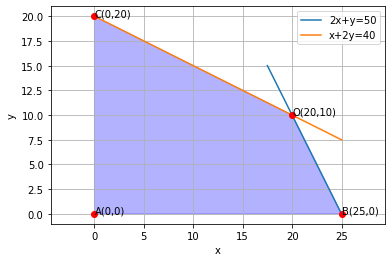
\includegraphics[width=\columnwidth]{solutions/su2021/2/13/Figure9.png}
\caption{Graphical Solution}
\label{opt/13/fig: Graphical Solution}	
\end{figure}


\item Construct an isosceles triangle whose base is $a=8$cm and altitude $AD=h=4$cm 
\\
\solution

\begin{table}[!ht]
\centering
\resizebox{\columnwidth}{!}{\begin{tabular}{|c|c|c|c|} 
\hline
kind of  cake & No.of cakes & Flour& Fat\\
\hline
1st & x & 200g  &  25g \\ 
\hline
2nd& y& 100g&  50g  \\ 
\hline
Total& x+y& 5 kg=5000g&1kg=1000g \\ 
\hline
\end{tabular}}
\caption{Ingredients used in making the cake is flour and fat }
\label{opt/13/tab:table1}
\end{table}
Let the  1st kind  be $x$ and the 2nd kind be $y$  such that 
\begin{align}
x \geq 0 \\
y \geq 0 
\end{align}
According to the question,
\begin{align}
2{x} + {y} \leq 50
\\
{x} + 2{y} \leq 40
\end{align}
$\therefore$ Our problem is
\begin{align}
\max_{\vec{x}} Z &= \myvec{1& 1}\vec{x}\\
s.t. \quad \myvec{2 & 1 \\ 1& 2}\vec{x} &\preceq \myvec{50\\40} 
\end{align}
Lagrangian function is given by
\begin{equation}
\begin{aligned}
&L(\vec{x},\boldsymbol{\lambda}) \\ &= \myvec{1 & 1}\vec{x}+\lcbrak{\sbrak{\myvec{2 & 1}\vec{x}-50}} \\ &+ \sbrak{\myvec{1 & 2}\vec{x}-40}\\ &+ \sbrak{\myvec{-1 & 0}\vec{x}} +\rcbrak{\sbrak{\myvec{0 & -1}\vec{x}}}\boldsymbol{\lambda}
\end{aligned}
\end{equation}
where,
\begin{align}
\boldsymbol{\lambda} &= \myvec{\lambda_1 \\ \lambda_2 \\ \lambda_3 \\ \lambda_4 \\ \lambda_5 \\ \lambda_6}
\end{align}
Now,
\begin{align}
\nabla L(\vec{x},\boldsymbol{\lambda}) &= \myvec{1+ \myvec{2 & 1 & -1 & 0 }\boldsymbol{\lambda}\\ 1+\myvec{1 & 2 & 0 & -1}\boldsymbol{\lambda} \\ \myvec{2 & 1}\vec{x}-50\\ \myvec{1& 2}\vec{x}-40 \\  \myvec{-1 & 0}\vec{x} \\ \myvec{0 & -1}\vec{x}}
\end{align}
$\therefore$ Lagrangian matrix is given by
\begin{align}
\myvec{0 & 0 & 2 & 1& -1 & 0 \\ 0 & 0 & 1 & 2  & 0 & -1 \\ 2 & 1 & 0 & 0 & 0 & 0 \\ 1 & 2 & 0 & 0 & 0 & 0  \\ -1 & 0 & 0 & 0 & 0 & 0  \\ 0 & -1 & 0 & 0 & 0 & 0 }\myvec{\vec{x} \\ \boldsymbol{\lambda} } &= \myvec{-1 \\ -1 \\ 50\\ 4 0\\ 0 \\0 }
\end{align}
Considering $\lambda_1,\lambda_2$ as only active multiplier,
\begin{align}
\myvec{0 & 0 & 2 & 1 \\ 0 & 0 & 1 & 2 \\ 2 & 1 & 0 & 0 \\ 1 & 2 & 0 & 0}\myvec{\vec{x}\\ \boldsymbol{\lambda}} &= \myvec{-1 \\ -1 \\ 5 0\\ 40}
\end{align}
resulting in,
\begin{align}
\myvec{\vec{x} \\ \boldsymbol{\lambda}} &= \myvec{0 & 0 & 2 & 1 \\ 0 & 0 & 1 & 2 \\ 2 & 1 & 0 & 0 \\ 1& 2 & 0 & 0}^{-1}\myvec{-1 \\ -1 \\ 50 \\ 40}
\\
\implies   \myvec{\vec{x} \\ \boldsymbol{\lambda}} &= \myvec{0 & 0 & \frac{2}{3} & \frac{-1}{3} \\ 0 & 0 & \frac{-1}{3} & \frac{2}{3} \\ \frac{2}{3} & \frac{-1}{3} & 0 & 0 \\ \frac{-1}{3} & \frac{2}{3} & 0 & 0}\myvec{-1 \\ -1 \\ 50 \\ 40}
\\
\implies \myvec{\vec{x} \\ \boldsymbol{\lambda}} &= \myvec{20 \\ 10 \\ -0.3 \\ -0.3 }
\end{align}
$\because \boldsymbol{\lambda}=\myvec{-0.3 \\ -0.3} \succ \vec{0} $
\\
$\therefore$ Optimal solution is given by
\begin{align}
    \vec{x} &= \myvec{20\\10} \\
    Z &= \myvec{1& 1}\vec{x} \\
    &= \myvec{1 & 1}\myvec{20 \\ 10} \\
    &= 60
\end{align}
By using cvxpy in python ,
\begin{align}
    \vec{x}=\myvec{20\\10}\\
    Z = 60
\end{align}
Hence No.of cakes \boxed{x=20} 1st kind and  .of cakes \boxed{y=10} 2nd kind should be used to maximum No. of cakes \boxed{Z=60}.  This is
verified in Fig. \ref{opt/13/fig: Graphical Solution}.	
%
\begin{figure}[!ht]
\centering
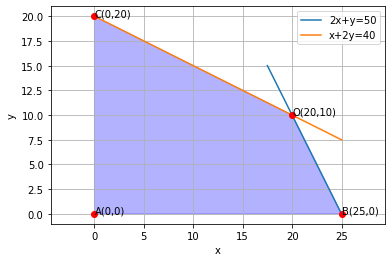
\includegraphics[width=\columnwidth]{solutions/su2021/2/13/Figure9.png}
\caption{Graphical Solution}
\label{opt/13/fig: Graphical Solution}	
\end{figure}


\item In $\triangle ABC$,  given that $a+b+c = 11, \angle B = 45^{\degree}$ and $\angle C = 45^{\degree}$, 
find 
$a,b,c$ and sketch the triangle.
\\
\solution

\begin{table}[!ht]
\centering
\resizebox{\columnwidth}{!}{\begin{tabular}{|c|c|c|c|} 
\hline
kind of  cake & No.of cakes & Flour& Fat\\
\hline
1st & x & 200g  &  25g \\ 
\hline
2nd& y& 100g&  50g  \\ 
\hline
Total& x+y& 5 kg=5000g&1kg=1000g \\ 
\hline
\end{tabular}}
\caption{Ingredients used in making the cake is flour and fat }
\label{opt/13/tab:table1}
\end{table}
Let the  1st kind  be $x$ and the 2nd kind be $y$  such that 
\begin{align}
x \geq 0 \\
y \geq 0 
\end{align}
According to the question,
\begin{align}
2{x} + {y} \leq 50
\\
{x} + 2{y} \leq 40
\end{align}
$\therefore$ Our problem is
\begin{align}
\max_{\vec{x}} Z &= \myvec{1& 1}\vec{x}\\
s.t. \quad \myvec{2 & 1 \\ 1& 2}\vec{x} &\preceq \myvec{50\\40} 
\end{align}
Lagrangian function is given by
\begin{equation}
\begin{aligned}
&L(\vec{x},\boldsymbol{\lambda}) \\ &= \myvec{1 & 1}\vec{x}+\lcbrak{\sbrak{\myvec{2 & 1}\vec{x}-50}} \\ &+ \sbrak{\myvec{1 & 2}\vec{x}-40}\\ &+ \sbrak{\myvec{-1 & 0}\vec{x}} +\rcbrak{\sbrak{\myvec{0 & -1}\vec{x}}}\boldsymbol{\lambda}
\end{aligned}
\end{equation}
where,
\begin{align}
\boldsymbol{\lambda} &= \myvec{\lambda_1 \\ \lambda_2 \\ \lambda_3 \\ \lambda_4 \\ \lambda_5 \\ \lambda_6}
\end{align}
Now,
\begin{align}
\nabla L(\vec{x},\boldsymbol{\lambda}) &= \myvec{1+ \myvec{2 & 1 & -1 & 0 }\boldsymbol{\lambda}\\ 1+\myvec{1 & 2 & 0 & -1}\boldsymbol{\lambda} \\ \myvec{2 & 1}\vec{x}-50\\ \myvec{1& 2}\vec{x}-40 \\  \myvec{-1 & 0}\vec{x} \\ \myvec{0 & -1}\vec{x}}
\end{align}
$\therefore$ Lagrangian matrix is given by
\begin{align}
\myvec{0 & 0 & 2 & 1& -1 & 0 \\ 0 & 0 & 1 & 2  & 0 & -1 \\ 2 & 1 & 0 & 0 & 0 & 0 \\ 1 & 2 & 0 & 0 & 0 & 0  \\ -1 & 0 & 0 & 0 & 0 & 0  \\ 0 & -1 & 0 & 0 & 0 & 0 }\myvec{\vec{x} \\ \boldsymbol{\lambda} } &= \myvec{-1 \\ -1 \\ 50\\ 4 0\\ 0 \\0 }
\end{align}
Considering $\lambda_1,\lambda_2$ as only active multiplier,
\begin{align}
\myvec{0 & 0 & 2 & 1 \\ 0 & 0 & 1 & 2 \\ 2 & 1 & 0 & 0 \\ 1 & 2 & 0 & 0}\myvec{\vec{x}\\ \boldsymbol{\lambda}} &= \myvec{-1 \\ -1 \\ 5 0\\ 40}
\end{align}
resulting in,
\begin{align}
\myvec{\vec{x} \\ \boldsymbol{\lambda}} &= \myvec{0 & 0 & 2 & 1 \\ 0 & 0 & 1 & 2 \\ 2 & 1 & 0 & 0 \\ 1& 2 & 0 & 0}^{-1}\myvec{-1 \\ -1 \\ 50 \\ 40}
\\
\implies   \myvec{\vec{x} \\ \boldsymbol{\lambda}} &= \myvec{0 & 0 & \frac{2}{3} & \frac{-1}{3} \\ 0 & 0 & \frac{-1}{3} & \frac{2}{3} \\ \frac{2}{3} & \frac{-1}{3} & 0 & 0 \\ \frac{-1}{3} & \frac{2}{3} & 0 & 0}\myvec{-1 \\ -1 \\ 50 \\ 40}
\\
\implies \myvec{\vec{x} \\ \boldsymbol{\lambda}} &= \myvec{20 \\ 10 \\ -0.3 \\ -0.3 }
\end{align}
$\because \boldsymbol{\lambda}=\myvec{-0.3 \\ -0.3} \succ \vec{0} $
\\
$\therefore$ Optimal solution is given by
\begin{align}
    \vec{x} &= \myvec{20\\10} \\
    Z &= \myvec{1& 1}\vec{x} \\
    &= \myvec{1 & 1}\myvec{20 \\ 10} \\
    &= 60
\end{align}
By using cvxpy in python ,
\begin{align}
    \vec{x}=\myvec{20\\10}\\
    Z = 60
\end{align}
Hence No.of cakes \boxed{x=20} 1st kind and  .of cakes \boxed{y=10} 2nd kind should be used to maximum No. of cakes \boxed{Z=60}.  This is
verified in Fig. \ref{opt/13/fig: Graphical Solution}.	
%
\begin{figure}[!ht]
\centering
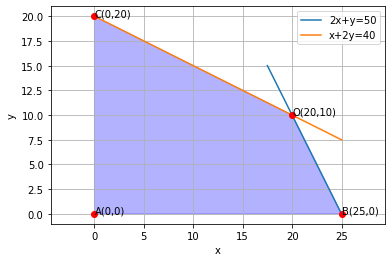
\includegraphics[width=\columnwidth]{solutions/su2021/2/13/Figure9.png}
\caption{Graphical Solution}
\label{opt/13/fig: Graphical Solution}	
\end{figure}


\item Draw $\triangle ABC$ with $a = 6, c = 5$ and $\angle B = 60 \degree$. 
\\
\solution

\begin{table}[!ht]
\centering
\resizebox{\columnwidth}{!}{\begin{tabular}{|c|c|c|c|} 
\hline
kind of  cake & No.of cakes & Flour& Fat\\
\hline
1st & x & 200g  &  25g \\ 
\hline
2nd& y& 100g&  50g  \\ 
\hline
Total& x+y& 5 kg=5000g&1kg=1000g \\ 
\hline
\end{tabular}}
\caption{Ingredients used in making the cake is flour and fat }
\label{opt/13/tab:table1}
\end{table}
Let the  1st kind  be $x$ and the 2nd kind be $y$  such that 
\begin{align}
x \geq 0 \\
y \geq 0 
\end{align}
According to the question,
\begin{align}
2{x} + {y} \leq 50
\\
{x} + 2{y} \leq 40
\end{align}
$\therefore$ Our problem is
\begin{align}
\max_{\vec{x}} Z &= \myvec{1& 1}\vec{x}\\
s.t. \quad \myvec{2 & 1 \\ 1& 2}\vec{x} &\preceq \myvec{50\\40} 
\end{align}
Lagrangian function is given by
\begin{equation}
\begin{aligned}
&L(\vec{x},\boldsymbol{\lambda}) \\ &= \myvec{1 & 1}\vec{x}+\lcbrak{\sbrak{\myvec{2 & 1}\vec{x}-50}} \\ &+ \sbrak{\myvec{1 & 2}\vec{x}-40}\\ &+ \sbrak{\myvec{-1 & 0}\vec{x}} +\rcbrak{\sbrak{\myvec{0 & -1}\vec{x}}}\boldsymbol{\lambda}
\end{aligned}
\end{equation}
where,
\begin{align}
\boldsymbol{\lambda} &= \myvec{\lambda_1 \\ \lambda_2 \\ \lambda_3 \\ \lambda_4 \\ \lambda_5 \\ \lambda_6}
\end{align}
Now,
\begin{align}
\nabla L(\vec{x},\boldsymbol{\lambda}) &= \myvec{1+ \myvec{2 & 1 & -1 & 0 }\boldsymbol{\lambda}\\ 1+\myvec{1 & 2 & 0 & -1}\boldsymbol{\lambda} \\ \myvec{2 & 1}\vec{x}-50\\ \myvec{1& 2}\vec{x}-40 \\  \myvec{-1 & 0}\vec{x} \\ \myvec{0 & -1}\vec{x}}
\end{align}
$\therefore$ Lagrangian matrix is given by
\begin{align}
\myvec{0 & 0 & 2 & 1& -1 & 0 \\ 0 & 0 & 1 & 2  & 0 & -1 \\ 2 & 1 & 0 & 0 & 0 & 0 \\ 1 & 2 & 0 & 0 & 0 & 0  \\ -1 & 0 & 0 & 0 & 0 & 0  \\ 0 & -1 & 0 & 0 & 0 & 0 }\myvec{\vec{x} \\ \boldsymbol{\lambda} } &= \myvec{-1 \\ -1 \\ 50\\ 4 0\\ 0 \\0 }
\end{align}
Considering $\lambda_1,\lambda_2$ as only active multiplier,
\begin{align}
\myvec{0 & 0 & 2 & 1 \\ 0 & 0 & 1 & 2 \\ 2 & 1 & 0 & 0 \\ 1 & 2 & 0 & 0}\myvec{\vec{x}\\ \boldsymbol{\lambda}} &= \myvec{-1 \\ -1 \\ 5 0\\ 40}
\end{align}
resulting in,
\begin{align}
\myvec{\vec{x} \\ \boldsymbol{\lambda}} &= \myvec{0 & 0 & 2 & 1 \\ 0 & 0 & 1 & 2 \\ 2 & 1 & 0 & 0 \\ 1& 2 & 0 & 0}^{-1}\myvec{-1 \\ -1 \\ 50 \\ 40}
\\
\implies   \myvec{\vec{x} \\ \boldsymbol{\lambda}} &= \myvec{0 & 0 & \frac{2}{3} & \frac{-1}{3} \\ 0 & 0 & \frac{-1}{3} & \frac{2}{3} \\ \frac{2}{3} & \frac{-1}{3} & 0 & 0 \\ \frac{-1}{3} & \frac{2}{3} & 0 & 0}\myvec{-1 \\ -1 \\ 50 \\ 40}
\\
\implies \myvec{\vec{x} \\ \boldsymbol{\lambda}} &= \myvec{20 \\ 10 \\ -0.3 \\ -0.3 }
\end{align}
$\because \boldsymbol{\lambda}=\myvec{-0.3 \\ -0.3} \succ \vec{0} $
\\
$\therefore$ Optimal solution is given by
\begin{align}
    \vec{x} &= \myvec{20\\10} \\
    Z &= \myvec{1& 1}\vec{x} \\
    &= \myvec{1 & 1}\myvec{20 \\ 10} \\
    &= 60
\end{align}
By using cvxpy in python ,
\begin{align}
    \vec{x}=\myvec{20\\10}\\
    Z = 60
\end{align}
Hence No.of cakes \boxed{x=20} 1st kind and  .of cakes \boxed{y=10} 2nd kind should be used to maximum No. of cakes \boxed{Z=60}.  This is
verified in Fig. \ref{opt/13/fig: Graphical Solution}.	
%
\begin{figure}[!ht]
\centering
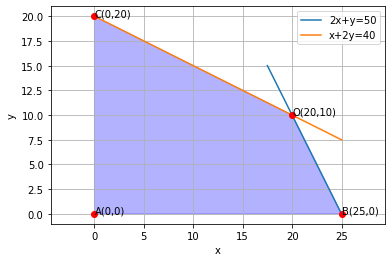
\includegraphics[width=\columnwidth]{solutions/su2021/2/13/Figure9.png}
\caption{Graphical Solution}
\label{opt/13/fig: Graphical Solution}	
\end{figure}


\item Draw $\triangle ABC$ with $a = 7, \angle B = 45\degree$ and $\angle A = 105 \degree$. 
\\
\solution

\begin{table}[!ht]
\centering
\resizebox{\columnwidth}{!}{\begin{tabular}{|c|c|c|c|} 
\hline
kind of  cake & No.of cakes & Flour& Fat\\
\hline
1st & x & 200g  &  25g \\ 
\hline
2nd& y& 100g&  50g  \\ 
\hline
Total& x+y& 5 kg=5000g&1kg=1000g \\ 
\hline
\end{tabular}}
\caption{Ingredients used in making the cake is flour and fat }
\label{opt/13/tab:table1}
\end{table}
Let the  1st kind  be $x$ and the 2nd kind be $y$  such that 
\begin{align}
x \geq 0 \\
y \geq 0 
\end{align}
According to the question,
\begin{align}
2{x} + {y} \leq 50
\\
{x} + 2{y} \leq 40
\end{align}
$\therefore$ Our problem is
\begin{align}
\max_{\vec{x}} Z &= \myvec{1& 1}\vec{x}\\
s.t. \quad \myvec{2 & 1 \\ 1& 2}\vec{x} &\preceq \myvec{50\\40} 
\end{align}
Lagrangian function is given by
\begin{equation}
\begin{aligned}
&L(\vec{x},\boldsymbol{\lambda}) \\ &= \myvec{1 & 1}\vec{x}+\lcbrak{\sbrak{\myvec{2 & 1}\vec{x}-50}} \\ &+ \sbrak{\myvec{1 & 2}\vec{x}-40}\\ &+ \sbrak{\myvec{-1 & 0}\vec{x}} +\rcbrak{\sbrak{\myvec{0 & -1}\vec{x}}}\boldsymbol{\lambda}
\end{aligned}
\end{equation}
where,
\begin{align}
\boldsymbol{\lambda} &= \myvec{\lambda_1 \\ \lambda_2 \\ \lambda_3 \\ \lambda_4 \\ \lambda_5 \\ \lambda_6}
\end{align}
Now,
\begin{align}
\nabla L(\vec{x},\boldsymbol{\lambda}) &= \myvec{1+ \myvec{2 & 1 & -1 & 0 }\boldsymbol{\lambda}\\ 1+\myvec{1 & 2 & 0 & -1}\boldsymbol{\lambda} \\ \myvec{2 & 1}\vec{x}-50\\ \myvec{1& 2}\vec{x}-40 \\  \myvec{-1 & 0}\vec{x} \\ \myvec{0 & -1}\vec{x}}
\end{align}
$\therefore$ Lagrangian matrix is given by
\begin{align}
\myvec{0 & 0 & 2 & 1& -1 & 0 \\ 0 & 0 & 1 & 2  & 0 & -1 \\ 2 & 1 & 0 & 0 & 0 & 0 \\ 1 & 2 & 0 & 0 & 0 & 0  \\ -1 & 0 & 0 & 0 & 0 & 0  \\ 0 & -1 & 0 & 0 & 0 & 0 }\myvec{\vec{x} \\ \boldsymbol{\lambda} } &= \myvec{-1 \\ -1 \\ 50\\ 4 0\\ 0 \\0 }
\end{align}
Considering $\lambda_1,\lambda_2$ as only active multiplier,
\begin{align}
\myvec{0 & 0 & 2 & 1 \\ 0 & 0 & 1 & 2 \\ 2 & 1 & 0 & 0 \\ 1 & 2 & 0 & 0}\myvec{\vec{x}\\ \boldsymbol{\lambda}} &= \myvec{-1 \\ -1 \\ 5 0\\ 40}
\end{align}
resulting in,
\begin{align}
\myvec{\vec{x} \\ \boldsymbol{\lambda}} &= \myvec{0 & 0 & 2 & 1 \\ 0 & 0 & 1 & 2 \\ 2 & 1 & 0 & 0 \\ 1& 2 & 0 & 0}^{-1}\myvec{-1 \\ -1 \\ 50 \\ 40}
\\
\implies   \myvec{\vec{x} \\ \boldsymbol{\lambda}} &= \myvec{0 & 0 & \frac{2}{3} & \frac{-1}{3} \\ 0 & 0 & \frac{-1}{3} & \frac{2}{3} \\ \frac{2}{3} & \frac{-1}{3} & 0 & 0 \\ \frac{-1}{3} & \frac{2}{3} & 0 & 0}\myvec{-1 \\ -1 \\ 50 \\ 40}
\\
\implies \myvec{\vec{x} \\ \boldsymbol{\lambda}} &= \myvec{20 \\ 10 \\ -0.3 \\ -0.3 }
\end{align}
$\because \boldsymbol{\lambda}=\myvec{-0.3 \\ -0.3} \succ \vec{0} $
\\
$\therefore$ Optimal solution is given by
\begin{align}
    \vec{x} &= \myvec{20\\10} \\
    Z &= \myvec{1& 1}\vec{x} \\
    &= \myvec{1 & 1}\myvec{20 \\ 10} \\
    &= 60
\end{align}
By using cvxpy in python ,
\begin{align}
    \vec{x}=\myvec{20\\10}\\
    Z = 60
\end{align}
Hence No.of cakes \boxed{x=20} 1st kind and  .of cakes \boxed{y=10} 2nd kind should be used to maximum No. of cakes \boxed{Z=60}.  This is
verified in Fig. \ref{opt/13/fig: Graphical Solution}.	
%
\begin{figure}[!ht]
\centering
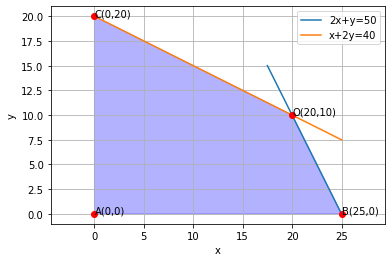
\includegraphics[width=\columnwidth]{solutions/su2021/2/13/Figure9.png}
\caption{Graphical Solution}
\label{opt/13/fig: Graphical Solution}	
\end{figure}


\item $\triangle ABC$ is right angled at $\vec{B}$.  If $a = 12$ and $b+c = 18$, find $b,c$ and draw the triangle.
\\
\solution

\begin{table}[!ht]
\centering
\resizebox{\columnwidth}{!}{\begin{tabular}{|c|c|c|c|} 
\hline
kind of  cake & No.of cakes & Flour& Fat\\
\hline
1st & x & 200g  &  25g \\ 
\hline
2nd& y& 100g&  50g  \\ 
\hline
Total& x+y& 5 kg=5000g&1kg=1000g \\ 
\hline
\end{tabular}}
\caption{Ingredients used in making the cake is flour and fat }
\label{opt/13/tab:table1}
\end{table}
Let the  1st kind  be $x$ and the 2nd kind be $y$  such that 
\begin{align}
x \geq 0 \\
y \geq 0 
\end{align}
According to the question,
\begin{align}
2{x} + {y} \leq 50
\\
{x} + 2{y} \leq 40
\end{align}
$\therefore$ Our problem is
\begin{align}
\max_{\vec{x}} Z &= \myvec{1& 1}\vec{x}\\
s.t. \quad \myvec{2 & 1 \\ 1& 2}\vec{x} &\preceq \myvec{50\\40} 
\end{align}
Lagrangian function is given by
\begin{equation}
\begin{aligned}
&L(\vec{x},\boldsymbol{\lambda}) \\ &= \myvec{1 & 1}\vec{x}+\lcbrak{\sbrak{\myvec{2 & 1}\vec{x}-50}} \\ &+ \sbrak{\myvec{1 & 2}\vec{x}-40}\\ &+ \sbrak{\myvec{-1 & 0}\vec{x}} +\rcbrak{\sbrak{\myvec{0 & -1}\vec{x}}}\boldsymbol{\lambda}
\end{aligned}
\end{equation}
where,
\begin{align}
\boldsymbol{\lambda} &= \myvec{\lambda_1 \\ \lambda_2 \\ \lambda_3 \\ \lambda_4 \\ \lambda_5 \\ \lambda_6}
\end{align}
Now,
\begin{align}
\nabla L(\vec{x},\boldsymbol{\lambda}) &= \myvec{1+ \myvec{2 & 1 & -1 & 0 }\boldsymbol{\lambda}\\ 1+\myvec{1 & 2 & 0 & -1}\boldsymbol{\lambda} \\ \myvec{2 & 1}\vec{x}-50\\ \myvec{1& 2}\vec{x}-40 \\  \myvec{-1 & 0}\vec{x} \\ \myvec{0 & -1}\vec{x}}
\end{align}
$\therefore$ Lagrangian matrix is given by
\begin{align}
\myvec{0 & 0 & 2 & 1& -1 & 0 \\ 0 & 0 & 1 & 2  & 0 & -1 \\ 2 & 1 & 0 & 0 & 0 & 0 \\ 1 & 2 & 0 & 0 & 0 & 0  \\ -1 & 0 & 0 & 0 & 0 & 0  \\ 0 & -1 & 0 & 0 & 0 & 0 }\myvec{\vec{x} \\ \boldsymbol{\lambda} } &= \myvec{-1 \\ -1 \\ 50\\ 4 0\\ 0 \\0 }
\end{align}
Considering $\lambda_1,\lambda_2$ as only active multiplier,
\begin{align}
\myvec{0 & 0 & 2 & 1 \\ 0 & 0 & 1 & 2 \\ 2 & 1 & 0 & 0 \\ 1 & 2 & 0 & 0}\myvec{\vec{x}\\ \boldsymbol{\lambda}} &= \myvec{-1 \\ -1 \\ 5 0\\ 40}
\end{align}
resulting in,
\begin{align}
\myvec{\vec{x} \\ \boldsymbol{\lambda}} &= \myvec{0 & 0 & 2 & 1 \\ 0 & 0 & 1 & 2 \\ 2 & 1 & 0 & 0 \\ 1& 2 & 0 & 0}^{-1}\myvec{-1 \\ -1 \\ 50 \\ 40}
\\
\implies   \myvec{\vec{x} \\ \boldsymbol{\lambda}} &= \myvec{0 & 0 & \frac{2}{3} & \frac{-1}{3} \\ 0 & 0 & \frac{-1}{3} & \frac{2}{3} \\ \frac{2}{3} & \frac{-1}{3} & 0 & 0 \\ \frac{-1}{3} & \frac{2}{3} & 0 & 0}\myvec{-1 \\ -1 \\ 50 \\ 40}
\\
\implies \myvec{\vec{x} \\ \boldsymbol{\lambda}} &= \myvec{20 \\ 10 \\ -0.3 \\ -0.3 }
\end{align}
$\because \boldsymbol{\lambda}=\myvec{-0.3 \\ -0.3} \succ \vec{0} $
\\
$\therefore$ Optimal solution is given by
\begin{align}
    \vec{x} &= \myvec{20\\10} \\
    Z &= \myvec{1& 1}\vec{x} \\
    &= \myvec{1 & 1}\myvec{20 \\ 10} \\
    &= 60
\end{align}
By using cvxpy in python ,
\begin{align}
    \vec{x}=\myvec{20\\10}\\
    Z = 60
\end{align}
Hence No.of cakes \boxed{x=20} 1st kind and  .of cakes \boxed{y=10} 2nd kind should be used to maximum No. of cakes \boxed{Z=60}.  This is
verified in Fig. \ref{opt/13/fig: Graphical Solution}.	
%
\begin{figure}[!ht]
\centering
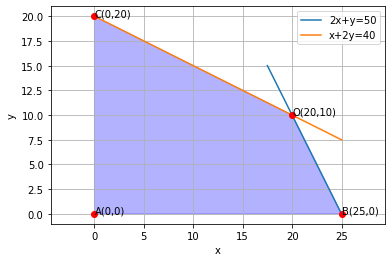
\includegraphics[width=\columnwidth]{solutions/su2021/2/13/Figure9.png}
\caption{Graphical Solution}
\label{opt/13/fig: Graphical Solution}	
\end{figure}

%\item Draw $\triangle ABC$ if $AB = 3, AC = 5$ and $\angle C = 30 \degree$.
\item In $\triangle ABC$,  $a = 8, \angle B = 45^{\degree}$ and $c-b = 3.5$.
Sketch $\triangle ABC$.
\\
\solution

\begin{table}[!ht]
\centering
\resizebox{\columnwidth}{!}{\begin{tabular}{|c|c|c|c|} 
\hline
kind of  cake & No.of cakes & Flour& Fat\\
\hline
1st & x & 200g  &  25g \\ 
\hline
2nd& y& 100g&  50g  \\ 
\hline
Total& x+y& 5 kg=5000g&1kg=1000g \\ 
\hline
\end{tabular}}
\caption{Ingredients used in making the cake is flour and fat }
\label{opt/13/tab:table1}
\end{table}
Let the  1st kind  be $x$ and the 2nd kind be $y$  such that 
\begin{align}
x \geq 0 \\
y \geq 0 
\end{align}
According to the question,
\begin{align}
2{x} + {y} \leq 50
\\
{x} + 2{y} \leq 40
\end{align}
$\therefore$ Our problem is
\begin{align}
\max_{\vec{x}} Z &= \myvec{1& 1}\vec{x}\\
s.t. \quad \myvec{2 & 1 \\ 1& 2}\vec{x} &\preceq \myvec{50\\40} 
\end{align}
Lagrangian function is given by
\begin{equation}
\begin{aligned}
&L(\vec{x},\boldsymbol{\lambda}) \\ &= \myvec{1 & 1}\vec{x}+\lcbrak{\sbrak{\myvec{2 & 1}\vec{x}-50}} \\ &+ \sbrak{\myvec{1 & 2}\vec{x}-40}\\ &+ \sbrak{\myvec{-1 & 0}\vec{x}} +\rcbrak{\sbrak{\myvec{0 & -1}\vec{x}}}\boldsymbol{\lambda}
\end{aligned}
\end{equation}
where,
\begin{align}
\boldsymbol{\lambda} &= \myvec{\lambda_1 \\ \lambda_2 \\ \lambda_3 \\ \lambda_4 \\ \lambda_5 \\ \lambda_6}
\end{align}
Now,
\begin{align}
\nabla L(\vec{x},\boldsymbol{\lambda}) &= \myvec{1+ \myvec{2 & 1 & -1 & 0 }\boldsymbol{\lambda}\\ 1+\myvec{1 & 2 & 0 & -1}\boldsymbol{\lambda} \\ \myvec{2 & 1}\vec{x}-50\\ \myvec{1& 2}\vec{x}-40 \\  \myvec{-1 & 0}\vec{x} \\ \myvec{0 & -1}\vec{x}}
\end{align}
$\therefore$ Lagrangian matrix is given by
\begin{align}
\myvec{0 & 0 & 2 & 1& -1 & 0 \\ 0 & 0 & 1 & 2  & 0 & -1 \\ 2 & 1 & 0 & 0 & 0 & 0 \\ 1 & 2 & 0 & 0 & 0 & 0  \\ -1 & 0 & 0 & 0 & 0 & 0  \\ 0 & -1 & 0 & 0 & 0 & 0 }\myvec{\vec{x} \\ \boldsymbol{\lambda} } &= \myvec{-1 \\ -1 \\ 50\\ 4 0\\ 0 \\0 }
\end{align}
Considering $\lambda_1,\lambda_2$ as only active multiplier,
\begin{align}
\myvec{0 & 0 & 2 & 1 \\ 0 & 0 & 1 & 2 \\ 2 & 1 & 0 & 0 \\ 1 & 2 & 0 & 0}\myvec{\vec{x}\\ \boldsymbol{\lambda}} &= \myvec{-1 \\ -1 \\ 5 0\\ 40}
\end{align}
resulting in,
\begin{align}
\myvec{\vec{x} \\ \boldsymbol{\lambda}} &= \myvec{0 & 0 & 2 & 1 \\ 0 & 0 & 1 & 2 \\ 2 & 1 & 0 & 0 \\ 1& 2 & 0 & 0}^{-1}\myvec{-1 \\ -1 \\ 50 \\ 40}
\\
\implies   \myvec{\vec{x} \\ \boldsymbol{\lambda}} &= \myvec{0 & 0 & \frac{2}{3} & \frac{-1}{3} \\ 0 & 0 & \frac{-1}{3} & \frac{2}{3} \\ \frac{2}{3} & \frac{-1}{3} & 0 & 0 \\ \frac{-1}{3} & \frac{2}{3} & 0 & 0}\myvec{-1 \\ -1 \\ 50 \\ 40}
\\
\implies \myvec{\vec{x} \\ \boldsymbol{\lambda}} &= \myvec{20 \\ 10 \\ -0.3 \\ -0.3 }
\end{align}
$\because \boldsymbol{\lambda}=\myvec{-0.3 \\ -0.3} \succ \vec{0} $
\\
$\therefore$ Optimal solution is given by
\begin{align}
    \vec{x} &= \myvec{20\\10} \\
    Z &= \myvec{1& 1}\vec{x} \\
    &= \myvec{1 & 1}\myvec{20 \\ 10} \\
    &= 60
\end{align}
By using cvxpy in python ,
\begin{align}
    \vec{x}=\myvec{20\\10}\\
    Z = 60
\end{align}
Hence No.of cakes \boxed{x=20} 1st kind and  .of cakes \boxed{y=10} 2nd kind should be used to maximum No. of cakes \boxed{Z=60}.  This is
verified in Fig. \ref{opt/13/fig: Graphical Solution}.	
%
\begin{figure}[!ht]
\centering
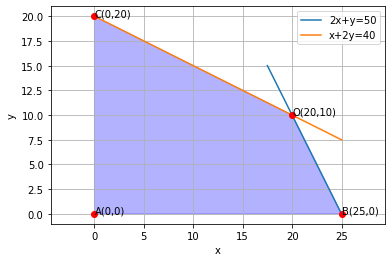
\includegraphics[width=\columnwidth]{solutions/su2021/2/13/Figure9.png}
\caption{Graphical Solution}
\label{opt/13/fig: Graphical Solution}	
\end{figure}


\item In $\triangle ABC$,  $a = 6, \angle B = 60^{\degree}$ and $b-c = 2$. 
Sketch $\triangle ABC$.

\begin{table}[!ht]
\centering
\resizebox{\columnwidth}{!}{\begin{tabular}{|c|c|c|c|} 
\hline
kind of  cake & No.of cakes & Flour& Fat\\
\hline
1st & x & 200g  &  25g \\ 
\hline
2nd& y& 100g&  50g  \\ 
\hline
Total& x+y& 5 kg=5000g&1kg=1000g \\ 
\hline
\end{tabular}}
\caption{Ingredients used in making the cake is flour and fat }
\label{opt/13/tab:table1}
\end{table}
Let the  1st kind  be $x$ and the 2nd kind be $y$  such that 
\begin{align}
x \geq 0 \\
y \geq 0 
\end{align}
According to the question,
\begin{align}
2{x} + {y} \leq 50
\\
{x} + 2{y} \leq 40
\end{align}
$\therefore$ Our problem is
\begin{align}
\max_{\vec{x}} Z &= \myvec{1& 1}\vec{x}\\
s.t. \quad \myvec{2 & 1 \\ 1& 2}\vec{x} &\preceq \myvec{50\\40} 
\end{align}
Lagrangian function is given by
\begin{equation}
\begin{aligned}
&L(\vec{x},\boldsymbol{\lambda}) \\ &= \myvec{1 & 1}\vec{x}+\lcbrak{\sbrak{\myvec{2 & 1}\vec{x}-50}} \\ &+ \sbrak{\myvec{1 & 2}\vec{x}-40}\\ &+ \sbrak{\myvec{-1 & 0}\vec{x}} +\rcbrak{\sbrak{\myvec{0 & -1}\vec{x}}}\boldsymbol{\lambda}
\end{aligned}
\end{equation}
where,
\begin{align}
\boldsymbol{\lambda} &= \myvec{\lambda_1 \\ \lambda_2 \\ \lambda_3 \\ \lambda_4 \\ \lambda_5 \\ \lambda_6}
\end{align}
Now,
\begin{align}
\nabla L(\vec{x},\boldsymbol{\lambda}) &= \myvec{1+ \myvec{2 & 1 & -1 & 0 }\boldsymbol{\lambda}\\ 1+\myvec{1 & 2 & 0 & -1}\boldsymbol{\lambda} \\ \myvec{2 & 1}\vec{x}-50\\ \myvec{1& 2}\vec{x}-40 \\  \myvec{-1 & 0}\vec{x} \\ \myvec{0 & -1}\vec{x}}
\end{align}
$\therefore$ Lagrangian matrix is given by
\begin{align}
\myvec{0 & 0 & 2 & 1& -1 & 0 \\ 0 & 0 & 1 & 2  & 0 & -1 \\ 2 & 1 & 0 & 0 & 0 & 0 \\ 1 & 2 & 0 & 0 & 0 & 0  \\ -1 & 0 & 0 & 0 & 0 & 0  \\ 0 & -1 & 0 & 0 & 0 & 0 }\myvec{\vec{x} \\ \boldsymbol{\lambda} } &= \myvec{-1 \\ -1 \\ 50\\ 4 0\\ 0 \\0 }
\end{align}
Considering $\lambda_1,\lambda_2$ as only active multiplier,
\begin{align}
\myvec{0 & 0 & 2 & 1 \\ 0 & 0 & 1 & 2 \\ 2 & 1 & 0 & 0 \\ 1 & 2 & 0 & 0}\myvec{\vec{x}\\ \boldsymbol{\lambda}} &= \myvec{-1 \\ -1 \\ 5 0\\ 40}
\end{align}
resulting in,
\begin{align}
\myvec{\vec{x} \\ \boldsymbol{\lambda}} &= \myvec{0 & 0 & 2 & 1 \\ 0 & 0 & 1 & 2 \\ 2 & 1 & 0 & 0 \\ 1& 2 & 0 & 0}^{-1}\myvec{-1 \\ -1 \\ 50 \\ 40}
\\
\implies   \myvec{\vec{x} \\ \boldsymbol{\lambda}} &= \myvec{0 & 0 & \frac{2}{3} & \frac{-1}{3} \\ 0 & 0 & \frac{-1}{3} & \frac{2}{3} \\ \frac{2}{3} & \frac{-1}{3} & 0 & 0 \\ \frac{-1}{3} & \frac{2}{3} & 0 & 0}\myvec{-1 \\ -1 \\ 50 \\ 40}
\\
\implies \myvec{\vec{x} \\ \boldsymbol{\lambda}} &= \myvec{20 \\ 10 \\ -0.3 \\ -0.3 }
\end{align}
$\because \boldsymbol{\lambda}=\myvec{-0.3 \\ -0.3} \succ \vec{0} $
\\
$\therefore$ Optimal solution is given by
\begin{align}
    \vec{x} &= \myvec{20\\10} \\
    Z &= \myvec{1& 1}\vec{x} \\
    &= \myvec{1 & 1}\myvec{20 \\ 10} \\
    &= 60
\end{align}
By using cvxpy in python ,
\begin{align}
    \vec{x}=\myvec{20\\10}\\
    Z = 60
\end{align}
Hence No.of cakes \boxed{x=20} 1st kind and  .of cakes \boxed{y=10} 2nd kind should be used to maximum No. of cakes \boxed{Z=60}.  This is
verified in Fig. \ref{opt/13/fig: Graphical Solution}.	
%
\begin{figure}[!ht]
\centering
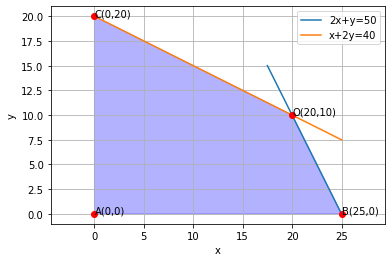
\includegraphics[width=\columnwidth]{solutions/su2021/2/13/Figure9.png}
\caption{Graphical Solution}
\label{opt/13/fig: Graphical Solution}	
\end{figure}

\item Draw $\triangle ABC$,  given that $a+b+c = 11, \angle B = 30^{\degree}$ and $\angle C = 90^{\degree}$.
\\
\solution

\begin{table}[!ht]
\centering
\resizebox{\columnwidth}{!}{\begin{tabular}{|c|c|c|c|} 
\hline
kind of  cake & No.of cakes & Flour& Fat\\
\hline
1st & x & 200g  &  25g \\ 
\hline
2nd& y& 100g&  50g  \\ 
\hline
Total& x+y& 5 kg=5000g&1kg=1000g \\ 
\hline
\end{tabular}}
\caption{Ingredients used in making the cake is flour and fat }
\label{opt/13/tab:table1}
\end{table}
Let the  1st kind  be $x$ and the 2nd kind be $y$  such that 
\begin{align}
x \geq 0 \\
y \geq 0 
\end{align}
According to the question,
\begin{align}
2{x} + {y} \leq 50
\\
{x} + 2{y} \leq 40
\end{align}
$\therefore$ Our problem is
\begin{align}
\max_{\vec{x}} Z &= \myvec{1& 1}\vec{x}\\
s.t. \quad \myvec{2 & 1 \\ 1& 2}\vec{x} &\preceq \myvec{50\\40} 
\end{align}
Lagrangian function is given by
\begin{equation}
\begin{aligned}
&L(\vec{x},\boldsymbol{\lambda}) \\ &= \myvec{1 & 1}\vec{x}+\lcbrak{\sbrak{\myvec{2 & 1}\vec{x}-50}} \\ &+ \sbrak{\myvec{1 & 2}\vec{x}-40}\\ &+ \sbrak{\myvec{-1 & 0}\vec{x}} +\rcbrak{\sbrak{\myvec{0 & -1}\vec{x}}}\boldsymbol{\lambda}
\end{aligned}
\end{equation}
where,
\begin{align}
\boldsymbol{\lambda} &= \myvec{\lambda_1 \\ \lambda_2 \\ \lambda_3 \\ \lambda_4 \\ \lambda_5 \\ \lambda_6}
\end{align}
Now,
\begin{align}
\nabla L(\vec{x},\boldsymbol{\lambda}) &= \myvec{1+ \myvec{2 & 1 & -1 & 0 }\boldsymbol{\lambda}\\ 1+\myvec{1 & 2 & 0 & -1}\boldsymbol{\lambda} \\ \myvec{2 & 1}\vec{x}-50\\ \myvec{1& 2}\vec{x}-40 \\  \myvec{-1 & 0}\vec{x} \\ \myvec{0 & -1}\vec{x}}
\end{align}
$\therefore$ Lagrangian matrix is given by
\begin{align}
\myvec{0 & 0 & 2 & 1& -1 & 0 \\ 0 & 0 & 1 & 2  & 0 & -1 \\ 2 & 1 & 0 & 0 & 0 & 0 \\ 1 & 2 & 0 & 0 & 0 & 0  \\ -1 & 0 & 0 & 0 & 0 & 0  \\ 0 & -1 & 0 & 0 & 0 & 0 }\myvec{\vec{x} \\ \boldsymbol{\lambda} } &= \myvec{-1 \\ -1 \\ 50\\ 4 0\\ 0 \\0 }
\end{align}
Considering $\lambda_1,\lambda_2$ as only active multiplier,
\begin{align}
\myvec{0 & 0 & 2 & 1 \\ 0 & 0 & 1 & 2 \\ 2 & 1 & 0 & 0 \\ 1 & 2 & 0 & 0}\myvec{\vec{x}\\ \boldsymbol{\lambda}} &= \myvec{-1 \\ -1 \\ 5 0\\ 40}
\end{align}
resulting in,
\begin{align}
\myvec{\vec{x} \\ \boldsymbol{\lambda}} &= \myvec{0 & 0 & 2 & 1 \\ 0 & 0 & 1 & 2 \\ 2 & 1 & 0 & 0 \\ 1& 2 & 0 & 0}^{-1}\myvec{-1 \\ -1 \\ 50 \\ 40}
\\
\implies   \myvec{\vec{x} \\ \boldsymbol{\lambda}} &= \myvec{0 & 0 & \frac{2}{3} & \frac{-1}{3} \\ 0 & 0 & \frac{-1}{3} & \frac{2}{3} \\ \frac{2}{3} & \frac{-1}{3} & 0 & 0 \\ \frac{-1}{3} & \frac{2}{3} & 0 & 0}\myvec{-1 \\ -1 \\ 50 \\ 40}
\\
\implies \myvec{\vec{x} \\ \boldsymbol{\lambda}} &= \myvec{20 \\ 10 \\ -0.3 \\ -0.3 }
\end{align}
$\because \boldsymbol{\lambda}=\myvec{-0.3 \\ -0.3} \succ \vec{0} $
\\
$\therefore$ Optimal solution is given by
\begin{align}
    \vec{x} &= \myvec{20\\10} \\
    Z &= \myvec{1& 1}\vec{x} \\
    &= \myvec{1 & 1}\myvec{20 \\ 10} \\
    &= 60
\end{align}
By using cvxpy in python ,
\begin{align}
    \vec{x}=\myvec{20\\10}\\
    Z = 60
\end{align}
Hence No.of cakes \boxed{x=20} 1st kind and  .of cakes \boxed{y=10} 2nd kind should be used to maximum No. of cakes \boxed{Z=60}.  This is
verified in Fig. \ref{opt/13/fig: Graphical Solution}.	
%
\begin{figure}[!ht]
\centering
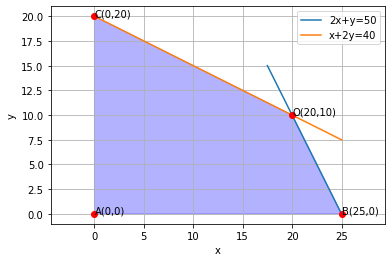
\includegraphics[width=\columnwidth]{solutions/su2021/2/13/Figure9.png}
\caption{Graphical Solution}
\label{opt/13/fig: Graphical Solution}	
\end{figure}


\item Construct $\triangle xyz$ where $xy = 4.5, yz = 5$ and $zx = 6$.
\\
\solution

\begin{table}[!ht]
\centering
\resizebox{\columnwidth}{!}{\begin{tabular}{|c|c|c|c|} 
\hline
kind of  cake & No.of cakes & Flour& Fat\\
\hline
1st & x & 200g  &  25g \\ 
\hline
2nd& y& 100g&  50g  \\ 
\hline
Total& x+y& 5 kg=5000g&1kg=1000g \\ 
\hline
\end{tabular}}
\caption{Ingredients used in making the cake is flour and fat }
\label{opt/13/tab:table1}
\end{table}
Let the  1st kind  be $x$ and the 2nd kind be $y$  such that 
\begin{align}
x \geq 0 \\
y \geq 0 
\end{align}
According to the question,
\begin{align}
2{x} + {y} \leq 50
\\
{x} + 2{y} \leq 40
\end{align}
$\therefore$ Our problem is
\begin{align}
\max_{\vec{x}} Z &= \myvec{1& 1}\vec{x}\\
s.t. \quad \myvec{2 & 1 \\ 1& 2}\vec{x} &\preceq \myvec{50\\40} 
\end{align}
Lagrangian function is given by
\begin{equation}
\begin{aligned}
&L(\vec{x},\boldsymbol{\lambda}) \\ &= \myvec{1 & 1}\vec{x}+\lcbrak{\sbrak{\myvec{2 & 1}\vec{x}-50}} \\ &+ \sbrak{\myvec{1 & 2}\vec{x}-40}\\ &+ \sbrak{\myvec{-1 & 0}\vec{x}} +\rcbrak{\sbrak{\myvec{0 & -1}\vec{x}}}\boldsymbol{\lambda}
\end{aligned}
\end{equation}
where,
\begin{align}
\boldsymbol{\lambda} &= \myvec{\lambda_1 \\ \lambda_2 \\ \lambda_3 \\ \lambda_4 \\ \lambda_5 \\ \lambda_6}
\end{align}
Now,
\begin{align}
\nabla L(\vec{x},\boldsymbol{\lambda}) &= \myvec{1+ \myvec{2 & 1 & -1 & 0 }\boldsymbol{\lambda}\\ 1+\myvec{1 & 2 & 0 & -1}\boldsymbol{\lambda} \\ \myvec{2 & 1}\vec{x}-50\\ \myvec{1& 2}\vec{x}-40 \\  \myvec{-1 & 0}\vec{x} \\ \myvec{0 & -1}\vec{x}}
\end{align}
$\therefore$ Lagrangian matrix is given by
\begin{align}
\myvec{0 & 0 & 2 & 1& -1 & 0 \\ 0 & 0 & 1 & 2  & 0 & -1 \\ 2 & 1 & 0 & 0 & 0 & 0 \\ 1 & 2 & 0 & 0 & 0 & 0  \\ -1 & 0 & 0 & 0 & 0 & 0  \\ 0 & -1 & 0 & 0 & 0 & 0 }\myvec{\vec{x} \\ \boldsymbol{\lambda} } &= \myvec{-1 \\ -1 \\ 50\\ 4 0\\ 0 \\0 }
\end{align}
Considering $\lambda_1,\lambda_2$ as only active multiplier,
\begin{align}
\myvec{0 & 0 & 2 & 1 \\ 0 & 0 & 1 & 2 \\ 2 & 1 & 0 & 0 \\ 1 & 2 & 0 & 0}\myvec{\vec{x}\\ \boldsymbol{\lambda}} &= \myvec{-1 \\ -1 \\ 5 0\\ 40}
\end{align}
resulting in,
\begin{align}
\myvec{\vec{x} \\ \boldsymbol{\lambda}} &= \myvec{0 & 0 & 2 & 1 \\ 0 & 0 & 1 & 2 \\ 2 & 1 & 0 & 0 \\ 1& 2 & 0 & 0}^{-1}\myvec{-1 \\ -1 \\ 50 \\ 40}
\\
\implies   \myvec{\vec{x} \\ \boldsymbol{\lambda}} &= \myvec{0 & 0 & \frac{2}{3} & \frac{-1}{3} \\ 0 & 0 & \frac{-1}{3} & \frac{2}{3} \\ \frac{2}{3} & \frac{-1}{3} & 0 & 0 \\ \frac{-1}{3} & \frac{2}{3} & 0 & 0}\myvec{-1 \\ -1 \\ 50 \\ 40}
\\
\implies \myvec{\vec{x} \\ \boldsymbol{\lambda}} &= \myvec{20 \\ 10 \\ -0.3 \\ -0.3 }
\end{align}
$\because \boldsymbol{\lambda}=\myvec{-0.3 \\ -0.3} \succ \vec{0} $
\\
$\therefore$ Optimal solution is given by
\begin{align}
    \vec{x} &= \myvec{20\\10} \\
    Z &= \myvec{1& 1}\vec{x} \\
    &= \myvec{1 & 1}\myvec{20 \\ 10} \\
    &= 60
\end{align}
By using cvxpy in python ,
\begin{align}
    \vec{x}=\myvec{20\\10}\\
    Z = 60
\end{align}
Hence No.of cakes \boxed{x=20} 1st kind and  .of cakes \boxed{y=10} 2nd kind should be used to maximum No. of cakes \boxed{Z=60}.  This is
verified in Fig. \ref{opt/13/fig: Graphical Solution}.	
%
\begin{figure}[!ht]
\centering
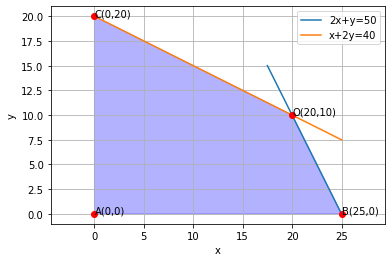
\includegraphics[width=\columnwidth]{solutions/su2021/2/13/Figure9.png}
\caption{Graphical Solution}
\label{opt/13/fig: Graphical Solution}	
\end{figure}


\item Draw an equilateral triangle of side $5.5$.
\\
\solution

\begin{table}[!ht]
\centering
\resizebox{\columnwidth}{!}{\begin{tabular}{|c|c|c|c|} 
\hline
kind of  cake & No.of cakes & Flour& Fat\\
\hline
1st & x & 200g  &  25g \\ 
\hline
2nd& y& 100g&  50g  \\ 
\hline
Total& x+y& 5 kg=5000g&1kg=1000g \\ 
\hline
\end{tabular}}
\caption{Ingredients used in making the cake is flour and fat }
\label{opt/13/tab:table1}
\end{table}
Let the  1st kind  be $x$ and the 2nd kind be $y$  such that 
\begin{align}
x \geq 0 \\
y \geq 0 
\end{align}
According to the question,
\begin{align}
2{x} + {y} \leq 50
\\
{x} + 2{y} \leq 40
\end{align}
$\therefore$ Our problem is
\begin{align}
\max_{\vec{x}} Z &= \myvec{1& 1}\vec{x}\\
s.t. \quad \myvec{2 & 1 \\ 1& 2}\vec{x} &\preceq \myvec{50\\40} 
\end{align}
Lagrangian function is given by
\begin{equation}
\begin{aligned}
&L(\vec{x},\boldsymbol{\lambda}) \\ &= \myvec{1 & 1}\vec{x}+\lcbrak{\sbrak{\myvec{2 & 1}\vec{x}-50}} \\ &+ \sbrak{\myvec{1 & 2}\vec{x}-40}\\ &+ \sbrak{\myvec{-1 & 0}\vec{x}} +\rcbrak{\sbrak{\myvec{0 & -1}\vec{x}}}\boldsymbol{\lambda}
\end{aligned}
\end{equation}
where,
\begin{align}
\boldsymbol{\lambda} &= \myvec{\lambda_1 \\ \lambda_2 \\ \lambda_3 \\ \lambda_4 \\ \lambda_5 \\ \lambda_6}
\end{align}
Now,
\begin{align}
\nabla L(\vec{x},\boldsymbol{\lambda}) &= \myvec{1+ \myvec{2 & 1 & -1 & 0 }\boldsymbol{\lambda}\\ 1+\myvec{1 & 2 & 0 & -1}\boldsymbol{\lambda} \\ \myvec{2 & 1}\vec{x}-50\\ \myvec{1& 2}\vec{x}-40 \\  \myvec{-1 & 0}\vec{x} \\ \myvec{0 & -1}\vec{x}}
\end{align}
$\therefore$ Lagrangian matrix is given by
\begin{align}
\myvec{0 & 0 & 2 & 1& -1 & 0 \\ 0 & 0 & 1 & 2  & 0 & -1 \\ 2 & 1 & 0 & 0 & 0 & 0 \\ 1 & 2 & 0 & 0 & 0 & 0  \\ -1 & 0 & 0 & 0 & 0 & 0  \\ 0 & -1 & 0 & 0 & 0 & 0 }\myvec{\vec{x} \\ \boldsymbol{\lambda} } &= \myvec{-1 \\ -1 \\ 50\\ 4 0\\ 0 \\0 }
\end{align}
Considering $\lambda_1,\lambda_2$ as only active multiplier,
\begin{align}
\myvec{0 & 0 & 2 & 1 \\ 0 & 0 & 1 & 2 \\ 2 & 1 & 0 & 0 \\ 1 & 2 & 0 & 0}\myvec{\vec{x}\\ \boldsymbol{\lambda}} &= \myvec{-1 \\ -1 \\ 5 0\\ 40}
\end{align}
resulting in,
\begin{align}
\myvec{\vec{x} \\ \boldsymbol{\lambda}} &= \myvec{0 & 0 & 2 & 1 \\ 0 & 0 & 1 & 2 \\ 2 & 1 & 0 & 0 \\ 1& 2 & 0 & 0}^{-1}\myvec{-1 \\ -1 \\ 50 \\ 40}
\\
\implies   \myvec{\vec{x} \\ \boldsymbol{\lambda}} &= \myvec{0 & 0 & \frac{2}{3} & \frac{-1}{3} \\ 0 & 0 & \frac{-1}{3} & \frac{2}{3} \\ \frac{2}{3} & \frac{-1}{3} & 0 & 0 \\ \frac{-1}{3} & \frac{2}{3} & 0 & 0}\myvec{-1 \\ -1 \\ 50 \\ 40}
\\
\implies \myvec{\vec{x} \\ \boldsymbol{\lambda}} &= \myvec{20 \\ 10 \\ -0.3 \\ -0.3 }
\end{align}
$\because \boldsymbol{\lambda}=\myvec{-0.3 \\ -0.3} \succ \vec{0} $
\\
$\therefore$ Optimal solution is given by
\begin{align}
    \vec{x} &= \myvec{20\\10} \\
    Z &= \myvec{1& 1}\vec{x} \\
    &= \myvec{1 & 1}\myvec{20 \\ 10} \\
    &= 60
\end{align}
By using cvxpy in python ,
\begin{align}
    \vec{x}=\myvec{20\\10}\\
    Z = 60
\end{align}
Hence No.of cakes \boxed{x=20} 1st kind and  .of cakes \boxed{y=10} 2nd kind should be used to maximum No. of cakes \boxed{Z=60}.  This is
verified in Fig. \ref{opt/13/fig: Graphical Solution}.	
%
\begin{figure}[!ht]
\centering
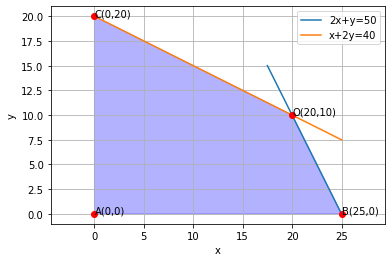
\includegraphics[width=\columnwidth]{solutions/su2021/2/13/Figure9.png}
\caption{Graphical Solution}
\label{opt/13/fig: Graphical Solution}	
\end{figure}


\item Draw $\triangle PQR$ with $PQ = 4, QR = 3.5$ and $PR = 4$.  What type of triangle is this?
\\
\solution

\begin{table}[!ht]
\centering
\resizebox{\columnwidth}{!}{\begin{tabular}{|c|c|c|c|} 
\hline
kind of  cake & No.of cakes & Flour& Fat\\
\hline
1st & x & 200g  &  25g \\ 
\hline
2nd& y& 100g&  50g  \\ 
\hline
Total& x+y& 5 kg=5000g&1kg=1000g \\ 
\hline
\end{tabular}}
\caption{Ingredients used in making the cake is flour and fat }
\label{opt/13/tab:table1}
\end{table}
Let the  1st kind  be $x$ and the 2nd kind be $y$  such that 
\begin{align}
x \geq 0 \\
y \geq 0 
\end{align}
According to the question,
\begin{align}
2{x} + {y} \leq 50
\\
{x} + 2{y} \leq 40
\end{align}
$\therefore$ Our problem is
\begin{align}
\max_{\vec{x}} Z &= \myvec{1& 1}\vec{x}\\
s.t. \quad \myvec{2 & 1 \\ 1& 2}\vec{x} &\preceq \myvec{50\\40} 
\end{align}
Lagrangian function is given by
\begin{equation}
\begin{aligned}
&L(\vec{x},\boldsymbol{\lambda}) \\ &= \myvec{1 & 1}\vec{x}+\lcbrak{\sbrak{\myvec{2 & 1}\vec{x}-50}} \\ &+ \sbrak{\myvec{1 & 2}\vec{x}-40}\\ &+ \sbrak{\myvec{-1 & 0}\vec{x}} +\rcbrak{\sbrak{\myvec{0 & -1}\vec{x}}}\boldsymbol{\lambda}
\end{aligned}
\end{equation}
where,
\begin{align}
\boldsymbol{\lambda} &= \myvec{\lambda_1 \\ \lambda_2 \\ \lambda_3 \\ \lambda_4 \\ \lambda_5 \\ \lambda_6}
\end{align}
Now,
\begin{align}
\nabla L(\vec{x},\boldsymbol{\lambda}) &= \myvec{1+ \myvec{2 & 1 & -1 & 0 }\boldsymbol{\lambda}\\ 1+\myvec{1 & 2 & 0 & -1}\boldsymbol{\lambda} \\ \myvec{2 & 1}\vec{x}-50\\ \myvec{1& 2}\vec{x}-40 \\  \myvec{-1 & 0}\vec{x} \\ \myvec{0 & -1}\vec{x}}
\end{align}
$\therefore$ Lagrangian matrix is given by
\begin{align}
\myvec{0 & 0 & 2 & 1& -1 & 0 \\ 0 & 0 & 1 & 2  & 0 & -1 \\ 2 & 1 & 0 & 0 & 0 & 0 \\ 1 & 2 & 0 & 0 & 0 & 0  \\ -1 & 0 & 0 & 0 & 0 & 0  \\ 0 & -1 & 0 & 0 & 0 & 0 }\myvec{\vec{x} \\ \boldsymbol{\lambda} } &= \myvec{-1 \\ -1 \\ 50\\ 4 0\\ 0 \\0 }
\end{align}
Considering $\lambda_1,\lambda_2$ as only active multiplier,
\begin{align}
\myvec{0 & 0 & 2 & 1 \\ 0 & 0 & 1 & 2 \\ 2 & 1 & 0 & 0 \\ 1 & 2 & 0 & 0}\myvec{\vec{x}\\ \boldsymbol{\lambda}} &= \myvec{-1 \\ -1 \\ 5 0\\ 40}
\end{align}
resulting in,
\begin{align}
\myvec{\vec{x} \\ \boldsymbol{\lambda}} &= \myvec{0 & 0 & 2 & 1 \\ 0 & 0 & 1 & 2 \\ 2 & 1 & 0 & 0 \\ 1& 2 & 0 & 0}^{-1}\myvec{-1 \\ -1 \\ 50 \\ 40}
\\
\implies   \myvec{\vec{x} \\ \boldsymbol{\lambda}} &= \myvec{0 & 0 & \frac{2}{3} & \frac{-1}{3} \\ 0 & 0 & \frac{-1}{3} & \frac{2}{3} \\ \frac{2}{3} & \frac{-1}{3} & 0 & 0 \\ \frac{-1}{3} & \frac{2}{3} & 0 & 0}\myvec{-1 \\ -1 \\ 50 \\ 40}
\\
\implies \myvec{\vec{x} \\ \boldsymbol{\lambda}} &= \myvec{20 \\ 10 \\ -0.3 \\ -0.3 }
\end{align}
$\because \boldsymbol{\lambda}=\myvec{-0.3 \\ -0.3} \succ \vec{0} $
\\
$\therefore$ Optimal solution is given by
\begin{align}
    \vec{x} &= \myvec{20\\10} \\
    Z &= \myvec{1& 1}\vec{x} \\
    &= \myvec{1 & 1}\myvec{20 \\ 10} \\
    &= 60
\end{align}
By using cvxpy in python ,
\begin{align}
    \vec{x}=\myvec{20\\10}\\
    Z = 60
\end{align}
Hence No.of cakes \boxed{x=20} 1st kind and  .of cakes \boxed{y=10} 2nd kind should be used to maximum No. of cakes \boxed{Z=60}.  This is
verified in Fig. \ref{opt/13/fig: Graphical Solution}.	
%
\begin{figure}[!ht]
\centering
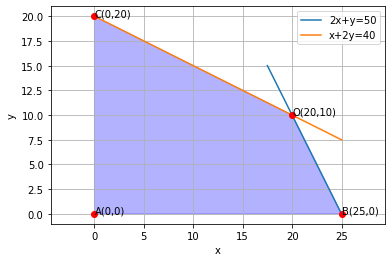
\includegraphics[width=\columnwidth]{solutions/su2021/2/13/Figure9.png}
\caption{Graphical Solution}
\label{opt/13/fig: Graphical Solution}	
\end{figure}


\item Construct $\triangle ABC$ such that $AB = 2.5, BC = 6$ and $AC = 6.5$.  Find $\angle B$.
\\
\solution

\begin{table}[!ht]
\centering
\resizebox{\columnwidth}{!}{\begin{tabular}{|c|c|c|c|} 
\hline
kind of  cake & No.of cakes & Flour& Fat\\
\hline
1st & x & 200g  &  25g \\ 
\hline
2nd& y& 100g&  50g  \\ 
\hline
Total& x+y& 5 kg=5000g&1kg=1000g \\ 
\hline
\end{tabular}}
\caption{Ingredients used in making the cake is flour and fat }
\label{opt/13/tab:table1}
\end{table}
Let the  1st kind  be $x$ and the 2nd kind be $y$  such that 
\begin{align}
x \geq 0 \\
y \geq 0 
\end{align}
According to the question,
\begin{align}
2{x} + {y} \leq 50
\\
{x} + 2{y} \leq 40
\end{align}
$\therefore$ Our problem is
\begin{align}
\max_{\vec{x}} Z &= \myvec{1& 1}\vec{x}\\
s.t. \quad \myvec{2 & 1 \\ 1& 2}\vec{x} &\preceq \myvec{50\\40} 
\end{align}
Lagrangian function is given by
\begin{equation}
\begin{aligned}
&L(\vec{x},\boldsymbol{\lambda}) \\ &= \myvec{1 & 1}\vec{x}+\lcbrak{\sbrak{\myvec{2 & 1}\vec{x}-50}} \\ &+ \sbrak{\myvec{1 & 2}\vec{x}-40}\\ &+ \sbrak{\myvec{-1 & 0}\vec{x}} +\rcbrak{\sbrak{\myvec{0 & -1}\vec{x}}}\boldsymbol{\lambda}
\end{aligned}
\end{equation}
where,
\begin{align}
\boldsymbol{\lambda} &= \myvec{\lambda_1 \\ \lambda_2 \\ \lambda_3 \\ \lambda_4 \\ \lambda_5 \\ \lambda_6}
\end{align}
Now,
\begin{align}
\nabla L(\vec{x},\boldsymbol{\lambda}) &= \myvec{1+ \myvec{2 & 1 & -1 & 0 }\boldsymbol{\lambda}\\ 1+\myvec{1 & 2 & 0 & -1}\boldsymbol{\lambda} \\ \myvec{2 & 1}\vec{x}-50\\ \myvec{1& 2}\vec{x}-40 \\  \myvec{-1 & 0}\vec{x} \\ \myvec{0 & -1}\vec{x}}
\end{align}
$\therefore$ Lagrangian matrix is given by
\begin{align}
\myvec{0 & 0 & 2 & 1& -1 & 0 \\ 0 & 0 & 1 & 2  & 0 & -1 \\ 2 & 1 & 0 & 0 & 0 & 0 \\ 1 & 2 & 0 & 0 & 0 & 0  \\ -1 & 0 & 0 & 0 & 0 & 0  \\ 0 & -1 & 0 & 0 & 0 & 0 }\myvec{\vec{x} \\ \boldsymbol{\lambda} } &= \myvec{-1 \\ -1 \\ 50\\ 4 0\\ 0 \\0 }
\end{align}
Considering $\lambda_1,\lambda_2$ as only active multiplier,
\begin{align}
\myvec{0 & 0 & 2 & 1 \\ 0 & 0 & 1 & 2 \\ 2 & 1 & 0 & 0 \\ 1 & 2 & 0 & 0}\myvec{\vec{x}\\ \boldsymbol{\lambda}} &= \myvec{-1 \\ -1 \\ 5 0\\ 40}
\end{align}
resulting in,
\begin{align}
\myvec{\vec{x} \\ \boldsymbol{\lambda}} &= \myvec{0 & 0 & 2 & 1 \\ 0 & 0 & 1 & 2 \\ 2 & 1 & 0 & 0 \\ 1& 2 & 0 & 0}^{-1}\myvec{-1 \\ -1 \\ 50 \\ 40}
\\
\implies   \myvec{\vec{x} \\ \boldsymbol{\lambda}} &= \myvec{0 & 0 & \frac{2}{3} & \frac{-1}{3} \\ 0 & 0 & \frac{-1}{3} & \frac{2}{3} \\ \frac{2}{3} & \frac{-1}{3} & 0 & 0 \\ \frac{-1}{3} & \frac{2}{3} & 0 & 0}\myvec{-1 \\ -1 \\ 50 \\ 40}
\\
\implies \myvec{\vec{x} \\ \boldsymbol{\lambda}} &= \myvec{20 \\ 10 \\ -0.3 \\ -0.3 }
\end{align}
$\because \boldsymbol{\lambda}=\myvec{-0.3 \\ -0.3} \succ \vec{0} $
\\
$\therefore$ Optimal solution is given by
\begin{align}
    \vec{x} &= \myvec{20\\10} \\
    Z &= \myvec{1& 1}\vec{x} \\
    &= \myvec{1 & 1}\myvec{20 \\ 10} \\
    &= 60
\end{align}
By using cvxpy in python ,
\begin{align}
    \vec{x}=\myvec{20\\10}\\
    Z = 60
\end{align}
Hence No.of cakes \boxed{x=20} 1st kind and  .of cakes \boxed{y=10} 2nd kind should be used to maximum No. of cakes \boxed{Z=60}.  This is
verified in Fig. \ref{opt/13/fig: Graphical Solution}.	
%
\begin{figure}[!ht]
\centering
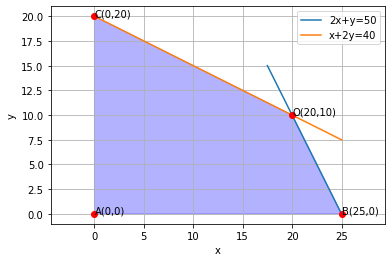
\includegraphics[width=\columnwidth]{solutions/su2021/2/13/Figure9.png}
\caption{Graphical Solution}
\label{opt/13/fig: Graphical Solution}	
\end{figure}


\item Construct $\triangle DEF$ such that $DE = 5, DF = 3$ and $\angle D = 90\degree$.
\\
\solution

\begin{table}[!ht]
\centering
\resizebox{\columnwidth}{!}{\begin{tabular}{|c|c|c|c|} 
\hline
kind of  cake & No.of cakes & Flour& Fat\\
\hline
1st & x & 200g  &  25g \\ 
\hline
2nd& y& 100g&  50g  \\ 
\hline
Total& x+y& 5 kg=5000g&1kg=1000g \\ 
\hline
\end{tabular}}
\caption{Ingredients used in making the cake is flour and fat }
\label{opt/13/tab:table1}
\end{table}
Let the  1st kind  be $x$ and the 2nd kind be $y$  such that 
\begin{align}
x \geq 0 \\
y \geq 0 
\end{align}
According to the question,
\begin{align}
2{x} + {y} \leq 50
\\
{x} + 2{y} \leq 40
\end{align}
$\therefore$ Our problem is
\begin{align}
\max_{\vec{x}} Z &= \myvec{1& 1}\vec{x}\\
s.t. \quad \myvec{2 & 1 \\ 1& 2}\vec{x} &\preceq \myvec{50\\40} 
\end{align}
Lagrangian function is given by
\begin{equation}
\begin{aligned}
&L(\vec{x},\boldsymbol{\lambda}) \\ &= \myvec{1 & 1}\vec{x}+\lcbrak{\sbrak{\myvec{2 & 1}\vec{x}-50}} \\ &+ \sbrak{\myvec{1 & 2}\vec{x}-40}\\ &+ \sbrak{\myvec{-1 & 0}\vec{x}} +\rcbrak{\sbrak{\myvec{0 & -1}\vec{x}}}\boldsymbol{\lambda}
\end{aligned}
\end{equation}
where,
\begin{align}
\boldsymbol{\lambda} &= \myvec{\lambda_1 \\ \lambda_2 \\ \lambda_3 \\ \lambda_4 \\ \lambda_5 \\ \lambda_6}
\end{align}
Now,
\begin{align}
\nabla L(\vec{x},\boldsymbol{\lambda}) &= \myvec{1+ \myvec{2 & 1 & -1 & 0 }\boldsymbol{\lambda}\\ 1+\myvec{1 & 2 & 0 & -1}\boldsymbol{\lambda} \\ \myvec{2 & 1}\vec{x}-50\\ \myvec{1& 2}\vec{x}-40 \\  \myvec{-1 & 0}\vec{x} \\ \myvec{0 & -1}\vec{x}}
\end{align}
$\therefore$ Lagrangian matrix is given by
\begin{align}
\myvec{0 & 0 & 2 & 1& -1 & 0 \\ 0 & 0 & 1 & 2  & 0 & -1 \\ 2 & 1 & 0 & 0 & 0 & 0 \\ 1 & 2 & 0 & 0 & 0 & 0  \\ -1 & 0 & 0 & 0 & 0 & 0  \\ 0 & -1 & 0 & 0 & 0 & 0 }\myvec{\vec{x} \\ \boldsymbol{\lambda} } &= \myvec{-1 \\ -1 \\ 50\\ 4 0\\ 0 \\0 }
\end{align}
Considering $\lambda_1,\lambda_2$ as only active multiplier,
\begin{align}
\myvec{0 & 0 & 2 & 1 \\ 0 & 0 & 1 & 2 \\ 2 & 1 & 0 & 0 \\ 1 & 2 & 0 & 0}\myvec{\vec{x}\\ \boldsymbol{\lambda}} &= \myvec{-1 \\ -1 \\ 5 0\\ 40}
\end{align}
resulting in,
\begin{align}
\myvec{\vec{x} \\ \boldsymbol{\lambda}} &= \myvec{0 & 0 & 2 & 1 \\ 0 & 0 & 1 & 2 \\ 2 & 1 & 0 & 0 \\ 1& 2 & 0 & 0}^{-1}\myvec{-1 \\ -1 \\ 50 \\ 40}
\\
\implies   \myvec{\vec{x} \\ \boldsymbol{\lambda}} &= \myvec{0 & 0 & \frac{2}{3} & \frac{-1}{3} \\ 0 & 0 & \frac{-1}{3} & \frac{2}{3} \\ \frac{2}{3} & \frac{-1}{3} & 0 & 0 \\ \frac{-1}{3} & \frac{2}{3} & 0 & 0}\myvec{-1 \\ -1 \\ 50 \\ 40}
\\
\implies \myvec{\vec{x} \\ \boldsymbol{\lambda}} &= \myvec{20 \\ 10 \\ -0.3 \\ -0.3 }
\end{align}
$\because \boldsymbol{\lambda}=\myvec{-0.3 \\ -0.3} \succ \vec{0} $
\\
$\therefore$ Optimal solution is given by
\begin{align}
    \vec{x} &= \myvec{20\\10} \\
    Z &= \myvec{1& 1}\vec{x} \\
    &= \myvec{1 & 1}\myvec{20 \\ 10} \\
    &= 60
\end{align}
By using cvxpy in python ,
\begin{align}
    \vec{x}=\myvec{20\\10}\\
    Z = 60
\end{align}
Hence No.of cakes \boxed{x=20} 1st kind and  .of cakes \boxed{y=10} 2nd kind should be used to maximum No. of cakes \boxed{Z=60}.  This is
verified in Fig. \ref{opt/13/fig: Graphical Solution}.	
%
\begin{figure}[!ht]
\centering
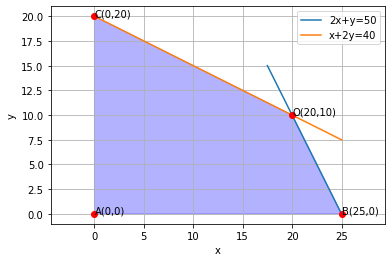
\includegraphics[width=\columnwidth]{solutions/su2021/2/13/Figure9.png}
\caption{Graphical Solution}
\label{opt/13/fig: Graphical Solution}	
\end{figure}


\item Construct an isosceles triangle in which the lengths of the equal sides is 6.5 and the angle between them is $110\degree$.
\\
\solution

\begin{table}[!ht]
\centering
\resizebox{\columnwidth}{!}{\begin{tabular}{|c|c|c|c|} 
\hline
kind of  cake & No.of cakes & Flour& Fat\\
\hline
1st & x & 200g  &  25g \\ 
\hline
2nd& y& 100g&  50g  \\ 
\hline
Total& x+y& 5 kg=5000g&1kg=1000g \\ 
\hline
\end{tabular}}
\caption{Ingredients used in making the cake is flour and fat }
\label{opt/13/tab:table1}
\end{table}
Let the  1st kind  be $x$ and the 2nd kind be $y$  such that 
\begin{align}
x \geq 0 \\
y \geq 0 
\end{align}
According to the question,
\begin{align}
2{x} + {y} \leq 50
\\
{x} + 2{y} \leq 40
\end{align}
$\therefore$ Our problem is
\begin{align}
\max_{\vec{x}} Z &= \myvec{1& 1}\vec{x}\\
s.t. \quad \myvec{2 & 1 \\ 1& 2}\vec{x} &\preceq \myvec{50\\40} 
\end{align}
Lagrangian function is given by
\begin{equation}
\begin{aligned}
&L(\vec{x},\boldsymbol{\lambda}) \\ &= \myvec{1 & 1}\vec{x}+\lcbrak{\sbrak{\myvec{2 & 1}\vec{x}-50}} \\ &+ \sbrak{\myvec{1 & 2}\vec{x}-40}\\ &+ \sbrak{\myvec{-1 & 0}\vec{x}} +\rcbrak{\sbrak{\myvec{0 & -1}\vec{x}}}\boldsymbol{\lambda}
\end{aligned}
\end{equation}
where,
\begin{align}
\boldsymbol{\lambda} &= \myvec{\lambda_1 \\ \lambda_2 \\ \lambda_3 \\ \lambda_4 \\ \lambda_5 \\ \lambda_6}
\end{align}
Now,
\begin{align}
\nabla L(\vec{x},\boldsymbol{\lambda}) &= \myvec{1+ \myvec{2 & 1 & -1 & 0 }\boldsymbol{\lambda}\\ 1+\myvec{1 & 2 & 0 & -1}\boldsymbol{\lambda} \\ \myvec{2 & 1}\vec{x}-50\\ \myvec{1& 2}\vec{x}-40 \\  \myvec{-1 & 0}\vec{x} \\ \myvec{0 & -1}\vec{x}}
\end{align}
$\therefore$ Lagrangian matrix is given by
\begin{align}
\myvec{0 & 0 & 2 & 1& -1 & 0 \\ 0 & 0 & 1 & 2  & 0 & -1 \\ 2 & 1 & 0 & 0 & 0 & 0 \\ 1 & 2 & 0 & 0 & 0 & 0  \\ -1 & 0 & 0 & 0 & 0 & 0  \\ 0 & -1 & 0 & 0 & 0 & 0 }\myvec{\vec{x} \\ \boldsymbol{\lambda} } &= \myvec{-1 \\ -1 \\ 50\\ 4 0\\ 0 \\0 }
\end{align}
Considering $\lambda_1,\lambda_2$ as only active multiplier,
\begin{align}
\myvec{0 & 0 & 2 & 1 \\ 0 & 0 & 1 & 2 \\ 2 & 1 & 0 & 0 \\ 1 & 2 & 0 & 0}\myvec{\vec{x}\\ \boldsymbol{\lambda}} &= \myvec{-1 \\ -1 \\ 5 0\\ 40}
\end{align}
resulting in,
\begin{align}
\myvec{\vec{x} \\ \boldsymbol{\lambda}} &= \myvec{0 & 0 & 2 & 1 \\ 0 & 0 & 1 & 2 \\ 2 & 1 & 0 & 0 \\ 1& 2 & 0 & 0}^{-1}\myvec{-1 \\ -1 \\ 50 \\ 40}
\\
\implies   \myvec{\vec{x} \\ \boldsymbol{\lambda}} &= \myvec{0 & 0 & \frac{2}{3} & \frac{-1}{3} \\ 0 & 0 & \frac{-1}{3} & \frac{2}{3} \\ \frac{2}{3} & \frac{-1}{3} & 0 & 0 \\ \frac{-1}{3} & \frac{2}{3} & 0 & 0}\myvec{-1 \\ -1 \\ 50 \\ 40}
\\
\implies \myvec{\vec{x} \\ \boldsymbol{\lambda}} &= \myvec{20 \\ 10 \\ -0.3 \\ -0.3 }
\end{align}
$\because \boldsymbol{\lambda}=\myvec{-0.3 \\ -0.3} \succ \vec{0} $
\\
$\therefore$ Optimal solution is given by
\begin{align}
    \vec{x} &= \myvec{20\\10} \\
    Z &= \myvec{1& 1}\vec{x} \\
    &= \myvec{1 & 1}\myvec{20 \\ 10} \\
    &= 60
\end{align}
By using cvxpy in python ,
\begin{align}
    \vec{x}=\myvec{20\\10}\\
    Z = 60
\end{align}
Hence No.of cakes \boxed{x=20} 1st kind and  .of cakes \boxed{y=10} 2nd kind should be used to maximum No. of cakes \boxed{Z=60}.  This is
verified in Fig. \ref{opt/13/fig: Graphical Solution}.	
%
\begin{figure}[!ht]
\centering
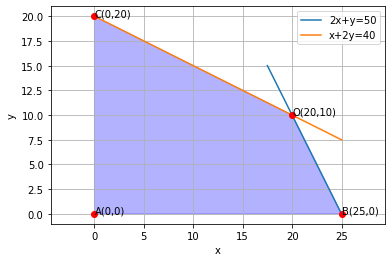
\includegraphics[width=\columnwidth]{solutions/su2021/2/13/Figure9.png}
\caption{Graphical Solution}
\label{opt/13/fig: Graphical Solution}	
\end{figure}

\item Construct $\triangle ABC$ given that $\angle A = 60\degree, \angle B = 30\degree$ and $AB = 5.8$.
\\
\solution
From the given information, 
\begin{align}
\angle C = 90^{\degree}
\end{align}
Hence, 
\begin{align}
\vec{A}&=\myvec{0\\c\sin{B}}\\
              &=\myvec{0\\2.9}\\
\vec{B} &=\myvec{c\cos{B}\\0}\\
               &=\myvec {5.02294\\0}\\
\vec{C} &=\myvec{0\\0}
\end{align}
which are used to draw $\triangle ABC$ in Fig. \ref{triangle/20/fig:triangle ABC}.
%
\begin{figure}[!ht]
\centering
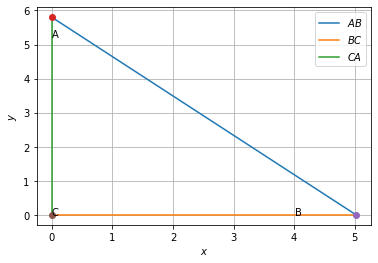
\includegraphics[width=\columnwidth]{solutions/triangle/20/Figure01.png}
\caption{$\triangle ABC$}
\label{triangle/20/fig:triangle ABC}
\end{figure}    

\item Construct  $\triangle LMN$ right angled at $M$ such that $LN = 5$ and $MN = 3$.
 \\
 \solution

\begin{table}[!ht]
\centering
\resizebox{\columnwidth}{!}{\begin{tabular}{|c|c|c|c|} 
\hline
kind of  cake & No.of cakes & Flour& Fat\\
\hline
1st & x & 200g  &  25g \\ 
\hline
2nd& y& 100g&  50g  \\ 
\hline
Total& x+y& 5 kg=5000g&1kg=1000g \\ 
\hline
\end{tabular}}
\caption{Ingredients used in making the cake is flour and fat }
\label{opt/13/tab:table1}
\end{table}
Let the  1st kind  be $x$ and the 2nd kind be $y$  such that 
\begin{align}
x \geq 0 \\
y \geq 0 
\end{align}
According to the question,
\begin{align}
2{x} + {y} \leq 50
\\
{x} + 2{y} \leq 40
\end{align}
$\therefore$ Our problem is
\begin{align}
\max_{\vec{x}} Z &= \myvec{1& 1}\vec{x}\\
s.t. \quad \myvec{2 & 1 \\ 1& 2}\vec{x} &\preceq \myvec{50\\40} 
\end{align}
Lagrangian function is given by
\begin{equation}
\begin{aligned}
&L(\vec{x},\boldsymbol{\lambda}) \\ &= \myvec{1 & 1}\vec{x}+\lcbrak{\sbrak{\myvec{2 & 1}\vec{x}-50}} \\ &+ \sbrak{\myvec{1 & 2}\vec{x}-40}\\ &+ \sbrak{\myvec{-1 & 0}\vec{x}} +\rcbrak{\sbrak{\myvec{0 & -1}\vec{x}}}\boldsymbol{\lambda}
\end{aligned}
\end{equation}
where,
\begin{align}
\boldsymbol{\lambda} &= \myvec{\lambda_1 \\ \lambda_2 \\ \lambda_3 \\ \lambda_4 \\ \lambda_5 \\ \lambda_6}
\end{align}
Now,
\begin{align}
\nabla L(\vec{x},\boldsymbol{\lambda}) &= \myvec{1+ \myvec{2 & 1 & -1 & 0 }\boldsymbol{\lambda}\\ 1+\myvec{1 & 2 & 0 & -1}\boldsymbol{\lambda} \\ \myvec{2 & 1}\vec{x}-50\\ \myvec{1& 2}\vec{x}-40 \\  \myvec{-1 & 0}\vec{x} \\ \myvec{0 & -1}\vec{x}}
\end{align}
$\therefore$ Lagrangian matrix is given by
\begin{align}
\myvec{0 & 0 & 2 & 1& -1 & 0 \\ 0 & 0 & 1 & 2  & 0 & -1 \\ 2 & 1 & 0 & 0 & 0 & 0 \\ 1 & 2 & 0 & 0 & 0 & 0  \\ -1 & 0 & 0 & 0 & 0 & 0  \\ 0 & -1 & 0 & 0 & 0 & 0 }\myvec{\vec{x} \\ \boldsymbol{\lambda} } &= \myvec{-1 \\ -1 \\ 50\\ 4 0\\ 0 \\0 }
\end{align}
Considering $\lambda_1,\lambda_2$ as only active multiplier,
\begin{align}
\myvec{0 & 0 & 2 & 1 \\ 0 & 0 & 1 & 2 \\ 2 & 1 & 0 & 0 \\ 1 & 2 & 0 & 0}\myvec{\vec{x}\\ \boldsymbol{\lambda}} &= \myvec{-1 \\ -1 \\ 5 0\\ 40}
\end{align}
resulting in,
\begin{align}
\myvec{\vec{x} \\ \boldsymbol{\lambda}} &= \myvec{0 & 0 & 2 & 1 \\ 0 & 0 & 1 & 2 \\ 2 & 1 & 0 & 0 \\ 1& 2 & 0 & 0}^{-1}\myvec{-1 \\ -1 \\ 50 \\ 40}
\\
\implies   \myvec{\vec{x} \\ \boldsymbol{\lambda}} &= \myvec{0 & 0 & \frac{2}{3} & \frac{-1}{3} \\ 0 & 0 & \frac{-1}{3} & \frac{2}{3} \\ \frac{2}{3} & \frac{-1}{3} & 0 & 0 \\ \frac{-1}{3} & \frac{2}{3} & 0 & 0}\myvec{-1 \\ -1 \\ 50 \\ 40}
\\
\implies \myvec{\vec{x} \\ \boldsymbol{\lambda}} &= \myvec{20 \\ 10 \\ -0.3 \\ -0.3 }
\end{align}
$\because \boldsymbol{\lambda}=\myvec{-0.3 \\ -0.3} \succ \vec{0} $
\\
$\therefore$ Optimal solution is given by
\begin{align}
    \vec{x} &= \myvec{20\\10} \\
    Z &= \myvec{1& 1}\vec{x} \\
    &= \myvec{1 & 1}\myvec{20 \\ 10} \\
    &= 60
\end{align}
By using cvxpy in python ,
\begin{align}
    \vec{x}=\myvec{20\\10}\\
    Z = 60
\end{align}
Hence No.of cakes \boxed{x=20} 1st kind and  .of cakes \boxed{y=10} 2nd kind should be used to maximum No. of cakes \boxed{Z=60}.  This is
verified in Fig. \ref{opt/13/fig: Graphical Solution}.	
%
\begin{figure}[!ht]
\centering
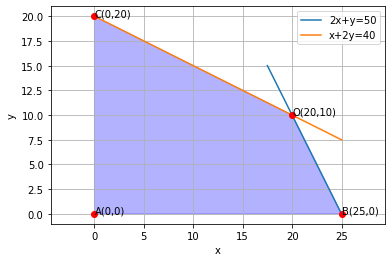
\includegraphics[width=\columnwidth]{solutions/su2021/2/13/Figure9.png}
\caption{Graphical Solution}
\label{opt/13/fig: Graphical Solution}	
\end{figure}

\item Construct  $\triangle PQR$ right angled at $Q$ such that $QR = 8$ and $PR = 10$.
\\
\solution
From the given information, 
\begin{align}
    \frac{AE}{EC} =  \frac{AD}{DB}&=\frac{1}{3}
\end{align}
and $\vec{D}$ divides AB in the ratio $1:3$ internally. $\vec{E}$ divides AE in the ratio $1:3$ internally.  Hence, 
\begin{align}
    \implies \vec{D} &=\frac{3\vec{A}+\vec{B}}{4}\\
    &=\myvec{\frac{13}{4}\\[2em]\frac{23}{4}}\\
    \vec{E} &=\frac{3\vec{A}+\vec{C}}{4}\\
    &=\myvec{\frac{19}{4}\\[2em]\frac{20}{4}}
\end{align}
\begin{align}
    \text{Area of } \triangle ABC &= \frac{1}{2}\norm{\brak{\vec{B-A}} \times \brak{\vec{C-A}}}\\
    &=\frac{1}{2}\norm{\myvec{-3\\-1}\times \myvec{3\\-4}}\\
        &=\frac{1}{2}\begin{vmatrix}
    -3&3\\
    -1&-4
    \end{vmatrix}\\
    &=\frac{1}{2}\sbrak{\brak{-3\times -4}-\brak{-1 \times 3}}\\
    &=\frac{15}{2}
\end{align}
\begin{align}
    \text{Area of } \triangle ADE &= \frac{1}{2}\norm{\brak{\vec{D-A}} \times \brak{\vec{E-A}}}\\
    &=\frac{1}{2}\norm{\myvec{\frac{-3}{4}\\[2em]\frac{-1}{4}}\times \myvec{\frac{3}{4}\\[2em]\frac{-4}{4}}}\\
    &=\frac{1}{2}\begin{vmatrix}
    \frac{-3}{4}&\frac{3}{4}\\[2em]
    \frac{-1}{4}&\frac{-4}{4}
    \end{vmatrix}\\
    &=\frac{1}{2}\sbrak{\brak{\frac{-3}{4}\times \frac{-4}{4}}-\brak{\frac{-1}{4} \times \frac{3}{4}}}\\
    &=\frac{15}{2\times16}
\end{align}
\begin{align}
    \frac{\text{area of } \triangle ADE}{\text{area of } \triangle ABC}=\frac{1}{16}
\end{align}
See Fig. \ref{aug/2/1plot}.
\begin{figure}[!h]
 \centering
 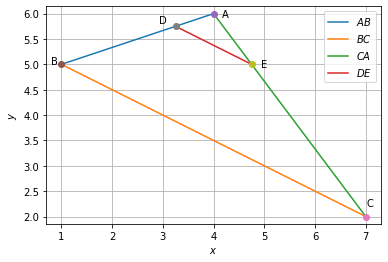
\includegraphics[width=\columnwidth]{solutions/aug/2/1/figs/figs.png}
 \caption{Plot of the triangles}
 \label{aug/2/1plot}
\end{figure}



\item Construct  right angled $\triangle $ whose hypotenuse  is 6 and one of the legs is 4.
\\
\solution
From the given information,
%
\begin{align}
\angle{C} = \ang{60}
\end{align}
%
Using the sine formula, 
%
\begin{align}
c &= b \brak{\frac{\sin{C}}{\sin{B}}} 
\\
&= 3.3915
\end{align}
%
the vertices of $\triangle ABC$ are
\begin{align}
\vec{A} = \myvec{0 \\ 0},
\vec{B} = c\myvec{\cos{\ang{70}} \\ \sin{\ang{70}}},
\vec{C} = \myvec{3 \\ 0}
\end{align}
and  plotted in Fig. \ref{constr/tri/27/3/fig:triangle ABC}.
%
\begin{figure}[ht]
    \centering
    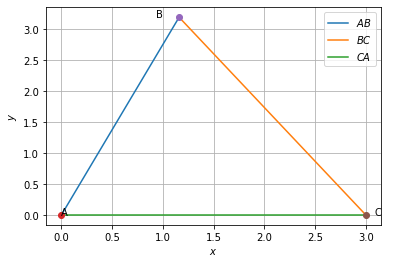
\includegraphics[width=\columnwidth]{solutions/triangle/27/3/Triangle_ABC.PNG}
    \caption{Plot of $\triangle ABC$}
    \label{constr/tri/27/3/fig:triangle ABC}
\end{figure}



\item Construct  an isosceles right angled $\triangle ABC$ right angled at $C$ such $AC = 6$.
\\
\solution

$\because \triangle ABC$ is isosceles, its vertices are
\begin{align}
\vec{C} = \myvec{0\\0},
\vec{A} = \myvec{6\\0}, 
\vec{B} = \myvec{0\\6}
\end{align}
which are used to plot the desired triangle in Fig. \ref{constr/26/fig:right_angle_triangle}.	
%
\begin{figure}[!ht]
\centering
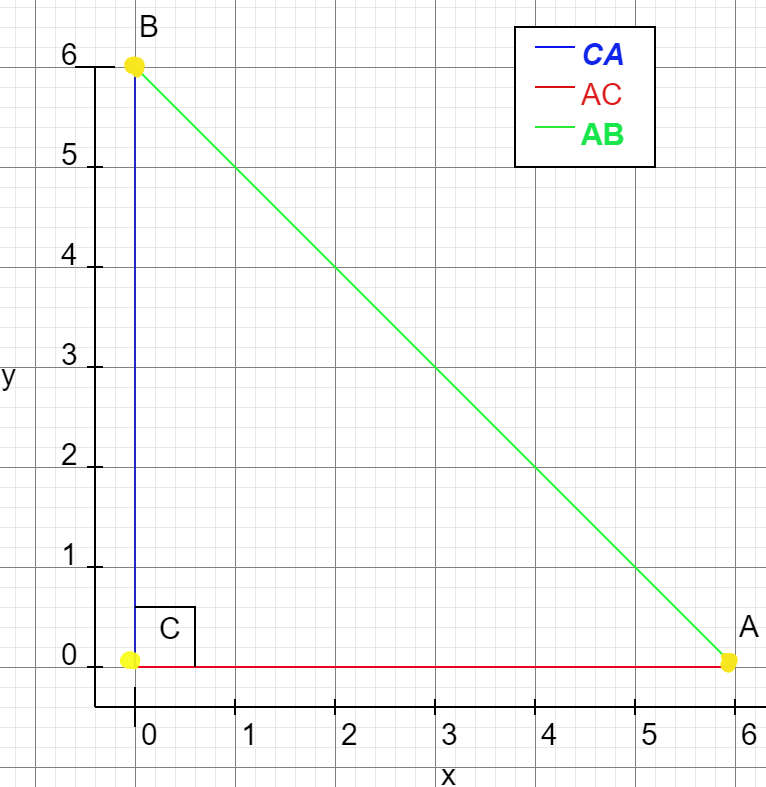
\includegraphics[width=\columnwidth]{solutions/26/diagram-1.png}
\caption{Isosceles Right Angle $\triangle ABC$}
\label{constr/26/fig:right_angle_triangle}	
\end{figure}



\item Construct $\triangle PQR$, given that $PQ = 3, QR = 5.5$ and $\angle PQR = 60 \degree$.
\\
\solution
\begin{align}
    \because \vec{P} = r\myvec{\cos Q\\ \sin Q}, \vec{Q} = \myvec{0\\0}, \vec{R} = \myvec{p\\0}
    \end{align}
    from the given information, 
    \begin{align}
    \vec{P} = 3\myvec{\cos60\\ \sin60} = \frac{3}{2}\myvec{1\\\sqrt3},  \vec{Q} = \myvec{0\\0},  \vec{R} = \myvec{5.5\\0}
    \end{align}
and plotted in Fig.              \ref{constr/july/1Figure}.
    
    
\begin{figure}[!ht]
\centering
         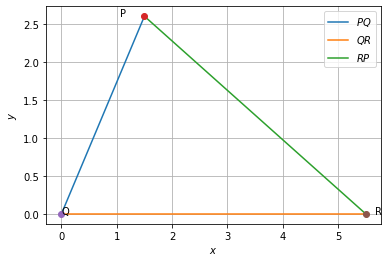
\includegraphics[width= \columnwidth]{solutions/july/2/1/figure1.png}
         \caption{The Constructed triangle}
         \label{constr/july/1Figure}
\end{figure}






%
\item Construct $\triangle ABC$  with $BC = 7.5, AC = 5$ and $\angle C = 60\degree$.
\\
\solution
From the given information, 
\begin{align}
    \frac{AE}{EC} =  \frac{AD}{DB}&=\frac{1}{3}
\end{align}
and $\vec{D}$ divides AB in the ratio $1:3$ internally. $\vec{E}$ divides AE in the ratio $1:3$ internally.  Hence, 
\begin{align}
    \implies \vec{D} &=\frac{3\vec{A}+\vec{B}}{4}\\
    &=\myvec{\frac{13}{4}\\[2em]\frac{23}{4}}\\
    \vec{E} &=\frac{3\vec{A}+\vec{C}}{4}\\
    &=\myvec{\frac{19}{4}\\[2em]\frac{20}{4}}
\end{align}
\begin{align}
    \text{Area of } \triangle ABC &= \frac{1}{2}\norm{\brak{\vec{B-A}} \times \brak{\vec{C-A}}}\\
    &=\frac{1}{2}\norm{\myvec{-3\\-1}\times \myvec{3\\-4}}\\
        &=\frac{1}{2}\begin{vmatrix}
    -3&3\\
    -1&-4
    \end{vmatrix}\\
    &=\frac{1}{2}\sbrak{\brak{-3\times -4}-\brak{-1 \times 3}}\\
    &=\frac{15}{2}
\end{align}
\begin{align}
    \text{Area of } \triangle ADE &= \frac{1}{2}\norm{\brak{\vec{D-A}} \times \brak{\vec{E-A}}}\\
    &=\frac{1}{2}\norm{\myvec{\frac{-3}{4}\\[2em]\frac{-1}{4}}\times \myvec{\frac{3}{4}\\[2em]\frac{-4}{4}}}\\
    &=\frac{1}{2}\begin{vmatrix}
    \frac{-3}{4}&\frac{3}{4}\\[2em]
    \frac{-1}{4}&\frac{-4}{4}
    \end{vmatrix}\\
    &=\frac{1}{2}\sbrak{\brak{\frac{-3}{4}\times \frac{-4}{4}}-\brak{\frac{-1}{4} \times \frac{3}{4}}}\\
    &=\frac{15}{2\times16}
\end{align}
\begin{align}
    \frac{\text{area of } \triangle ADE}{\text{area of } \triangle ABC}=\frac{1}{16}
\end{align}
See Fig. \ref{aug/2/1plot}.
\begin{figure}[!h]
 \centering
 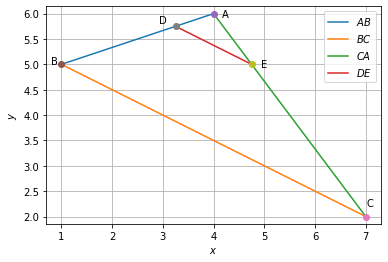
\includegraphics[width=\columnwidth]{solutions/aug/2/1/figs/figs.png}
 \caption{Plot of the triangles}
 \label{aug/2/1plot}
\end{figure}



\item Construct $\triangle XYZ$ if $XY = 6, \angle X = 30\degree$ and $\angle Y = 100 \degree$.
\\
\solution
Let
%
\begin{align}
 XY=z,  YZ=x,  XZ=y
\end{align}
From the given information,
%
\begin{align}
y&= z\brak{\frac{\sin{Y}}{\sin{Z}}} 
&= 6 \brak{\frac{\sin{\ang{100}}}{\sin{\ang{50}}}}
&= 7.7134
\end{align}
and the vertices are
\begin{align}
\vec{X} &= \myvec{\ 0\\ 0}, \vec{Y} = z\myvec{ \cos X\si{\degree}\\ \sin X\si{\degree}} ,\vec{Z} =\myvec{y \\ 0} \\
\\
\implies \vec{X} &=\myvec{0 \\ 0},
\vec{Y} =6\myvec{\cos{\ang{30}} \\ \sin{\ang{30}}} &= \myvec{3\sqrt{3} \\ 3 }, 
\vec{Z} =\myvec{7.7134 \\ 0}
\end{align}
and plotted in Fig. \ref{july/2/3/Figure}.
%
\begin{figure}[!b]
  \centering
            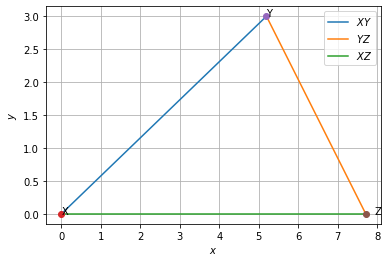
\includegraphics[width=\columnwidth]{solutions/july/2/3/Figure_1.png}
            \caption{Constructed Triangle}
            \label{july/2/3/Figure}
 \end{figure}
 %
 



\item If $AC = 7, \angle A = 60\degree$ and $\angle B = 50 \degree$, can you draw the triangle?
%
\\
\solution
\begin{equation}
\vec{a^Tb}=\myvec{3&-4&5} \myvec{-2\\1\\-3}  
\end{equation}
\begin{equation}
=(3\times -2)+(-4\times 1)+(5\times -3)
\end{equation}
\begin{equation}
=-25    
\end{equation}

\begin{equation}
\vec{a \times b} &= \myvec{0 & 5 & -4\\ 5 & 0 & -3\\ -(-4) & 3 &  0} \myvec{-2\\1\\3}    
\end{equation}
\\
\begin{equation}
\vec{a \times b}  =  \myvec{(0 \times -2)  +  (-5 \times 1)  +  (-4 \times -3)\\(5 \times -2)  +  (0 \times 1)  +  (-3 \times -3)\\(4 \times -2)  +  (3 \times 1)  + (0 \times -3)}    
\end{equation}
\\
\begin{equation}
\vec{a \times b}  =  \myvec{7\\-1\\5}    
\end{equation}


\item Construct $\triangle PQR$ if $PQ = 5, \angle Q = 105 \degree$ and $\angle R = 40 \degree$.
\\

\begin{table}[!ht]
\centering
\resizebox{\columnwidth}{!}{\begin{tabular}{|c|c|c|c|} 
\hline
kind of  cake & No.of cakes & Flour& Fat\\
\hline
1st & x & 200g  &  25g \\ 
\hline
2nd& y& 100g&  50g  \\ 
\hline
Total& x+y& 5 kg=5000g&1kg=1000g \\ 
\hline
\end{tabular}}
\caption{Ingredients used in making the cake is flour and fat }
\label{opt/13/tab:table1}
\end{table}
Let the  1st kind  be $x$ and the 2nd kind be $y$  such that 
\begin{align}
x \geq 0 \\
y \geq 0 
\end{align}
According to the question,
\begin{align}
2{x} + {y} \leq 50
\\
{x} + 2{y} \leq 40
\end{align}
$\therefore$ Our problem is
\begin{align}
\max_{\vec{x}} Z &= \myvec{1& 1}\vec{x}\\
s.t. \quad \myvec{2 & 1 \\ 1& 2}\vec{x} &\preceq \myvec{50\\40} 
\end{align}
Lagrangian function is given by
\begin{equation}
\begin{aligned}
&L(\vec{x},\boldsymbol{\lambda}) \\ &= \myvec{1 & 1}\vec{x}+\lcbrak{\sbrak{\myvec{2 & 1}\vec{x}-50}} \\ &+ \sbrak{\myvec{1 & 2}\vec{x}-40}\\ &+ \sbrak{\myvec{-1 & 0}\vec{x}} +\rcbrak{\sbrak{\myvec{0 & -1}\vec{x}}}\boldsymbol{\lambda}
\end{aligned}
\end{equation}
where,
\begin{align}
\boldsymbol{\lambda} &= \myvec{\lambda_1 \\ \lambda_2 \\ \lambda_3 \\ \lambda_4 \\ \lambda_5 \\ \lambda_6}
\end{align}
Now,
\begin{align}
\nabla L(\vec{x},\boldsymbol{\lambda}) &= \myvec{1+ \myvec{2 & 1 & -1 & 0 }\boldsymbol{\lambda}\\ 1+\myvec{1 & 2 & 0 & -1}\boldsymbol{\lambda} \\ \myvec{2 & 1}\vec{x}-50\\ \myvec{1& 2}\vec{x}-40 \\  \myvec{-1 & 0}\vec{x} \\ \myvec{0 & -1}\vec{x}}
\end{align}
$\therefore$ Lagrangian matrix is given by
\begin{align}
\myvec{0 & 0 & 2 & 1& -1 & 0 \\ 0 & 0 & 1 & 2  & 0 & -1 \\ 2 & 1 & 0 & 0 & 0 & 0 \\ 1 & 2 & 0 & 0 & 0 & 0  \\ -1 & 0 & 0 & 0 & 0 & 0  \\ 0 & -1 & 0 & 0 & 0 & 0 }\myvec{\vec{x} \\ \boldsymbol{\lambda} } &= \myvec{-1 \\ -1 \\ 50\\ 4 0\\ 0 \\0 }
\end{align}
Considering $\lambda_1,\lambda_2$ as only active multiplier,
\begin{align}
\myvec{0 & 0 & 2 & 1 \\ 0 & 0 & 1 & 2 \\ 2 & 1 & 0 & 0 \\ 1 & 2 & 0 & 0}\myvec{\vec{x}\\ \boldsymbol{\lambda}} &= \myvec{-1 \\ -1 \\ 5 0\\ 40}
\end{align}
resulting in,
\begin{align}
\myvec{\vec{x} \\ \boldsymbol{\lambda}} &= \myvec{0 & 0 & 2 & 1 \\ 0 & 0 & 1 & 2 \\ 2 & 1 & 0 & 0 \\ 1& 2 & 0 & 0}^{-1}\myvec{-1 \\ -1 \\ 50 \\ 40}
\\
\implies   \myvec{\vec{x} \\ \boldsymbol{\lambda}} &= \myvec{0 & 0 & \frac{2}{3} & \frac{-1}{3} \\ 0 & 0 & \frac{-1}{3} & \frac{2}{3} \\ \frac{2}{3} & \frac{-1}{3} & 0 & 0 \\ \frac{-1}{3} & \frac{2}{3} & 0 & 0}\myvec{-1 \\ -1 \\ 50 \\ 40}
\\
\implies \myvec{\vec{x} \\ \boldsymbol{\lambda}} &= \myvec{20 \\ 10 \\ -0.3 \\ -0.3 }
\end{align}
$\because \boldsymbol{\lambda}=\myvec{-0.3 \\ -0.3} \succ \vec{0} $
\\
$\therefore$ Optimal solution is given by
\begin{align}
    \vec{x} &= \myvec{20\\10} \\
    Z &= \myvec{1& 1}\vec{x} \\
    &= \myvec{1 & 1}\myvec{20 \\ 10} \\
    &= 60
\end{align}
By using cvxpy in python ,
\begin{align}
    \vec{x}=\myvec{20\\10}\\
    Z = 60
\end{align}
Hence No.of cakes \boxed{x=20} 1st kind and  .of cakes \boxed{y=10} 2nd kind should be used to maximum No. of cakes \boxed{Z=60}.  This is
verified in Fig. \ref{opt/13/fig: Graphical Solution}.	
%
\begin{figure}[!ht]
\centering
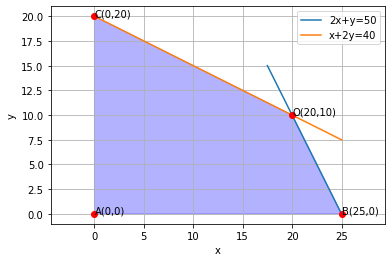
\includegraphics[width=\columnwidth]{solutions/su2021/2/13/Figure9.png}
\caption{Graphical Solution}
\label{opt/13/fig: Graphical Solution}	
\end{figure}

\item Can you construct $\triangle DEF$ such that $EF = 7.2, \angle E = 110\degree$ and $\angle F = 180\degree$?



%\end{enumerate}

